In Chapter \ref{ch:SpeciesIntro} we explained the central role of the species cut-off $\LSP$ as the energy scale controlling the maximum regime of validity of any effective field theory weakly coupled to Einstein gravity. Therefore, an interesting avenue to infer generic properties of quantum gravity, as seen from the low energy realm, involves systematically studying the behaviour of this energy scale across the landscape of consistent EFTs. In addition, this strategy would perhaps even allow us to obtain non-trivial information about yet unknown consistency conditions that must be generically satisfied in quantum gravity, and formulate them in the form of new universal constraints. To do so, a good starting point would be to analyze the behaviour of the QG cut-off close to infinite distance boundaries of moduli space, where many Swampland criteria have been already proposed and thoroughly tested (see Section \ref{s:SwamplandProgram} for details). In particular, the connection between the Swampland program and the species scale becomes very apparent when focusing on those consistency conditions which are formulated as continuous statements, such as the (sub-)Lattice/tower Weak Gravity Conjecture \cite{Heidenreich:2015nta,Heidenreich:2016aqi,Montero:2016tif,Andriolo:2018lvp} or the Distance Conjecture \cite{Ooguri:2006in, Etheredge:2022opl}. Indeed, these criteria usually deal with extreme regimes in the parameter (or moduli) space of low energy EFTs, where certain gauge couplings are taken to be close to zero value or rather we allow for enormous vacuum expectation values in the scalar fields; and the way in which these are censored is via the appearance of an infinite number of light states. This latter fact implies, in turn, that there should be a significant decrease of the species cut-off $\LSP$, such that the regime of validity of our starting effective description shrinks to the point in which it actually becomes completely invalidated (i.e. when sitting precisely at the infinite distance boundary).

The purpose of the present chapter is to revisit these considerations so as to propose, based several bottom-up arguments, a very sharp and universal \emph{lower bound} on the exponential decay rate, $\lambda_{\rm sp}$, of the quantum gravity cut-off (see Section \ref{s:convexhull} below for a precise definition of $\lambda_{\rm sp}$). More concretely, such constraint would read as follows
%
\begin{equation}\label{eq:lowerboundspecies}
  \lambda_{\rm sp} \geq \frac{1}{\sqrt{(d-1)(d-2)}}\, ,
\end{equation}
%
where $d$ denotes the spacetime dimension of our theory, and it should hold when venturing towards the boundaries of moduli space, regardless of the particular infinite distance limit that we choose to sample. We will thus first motivate the existence of the lower bound \eqref{eq:lowerboundspecies} in Section \ref{s:convexhull}, using our experience with string theory to guide us.\footnote{See also \cite{Calderon-Infante:2023ler} for complementary bottom-up arguments.} In practice, it may become highly involved to check the proposed bound, especially in the presence of several scalar fields, where the number of infinite distance singularities and relevant towers of states can easily proliferate. To sidestep this difficulty, we can reformulate the constraint \eqref{eq:lowerboundspecies} in terms of a convex hull condition, which is considerably easier to analyze. Later on, in Section \ref{s:consistencydimreduc}, we will study the stability (or consistency) of the lower bound under dimensional reduction. This analysis will moreover highlight the role of the saturating value $\lambda_{\rm sp,\, min} = \frac{1}{\sqrt{(d-1)(d-2)}}$, which actually arises in explicit examples such as $\mathbf{S}^1$--\,compactifications, as being the only one which is both preserved and consistent under the compactification process. Finally, we present top-down evidence for the bound \eqref{eq:lowerboundspecies} in Section \ref{s:examplesbound}, restricting to the case of maximal supergravity in $d\geq4$. Further non-trivial evidence for the latter in set-ups preserving less amount of supersymmetry will be provided in Chapter \ref{ch:pattern} below.

This chapter is based on the publication \cite{Calderon-Infante:2023ler}, which has been adapted to better fit in the broader context of this thesis.

\section{A convex hull condition for the species scale}
\label{s:convexhull}

We consider in the following a $d$-dimensional EFT containing a set of massless scalar fields (i.e. moduli), weakly coupled to Einstein gravity as follows
%
\begin{equation}\label{eq:action}
	\mathcal{L}_{\text{EFT}} \supset \dfrac{1}{2\kappa_d^2}\,  \sqrt{- g} \left(\mathcal{R} + G_{i j} (\phi)\, \partial \phi^i \cdot \partial \phi^j\right)\, ,
\end{equation}
%
where $G_{ij}(\phi)$ is the metric tensor associated to the moduli space, $\mathcal{M}_{\phi}$, spanned by the vacuum expectation values (v.e.v.s) of the massless scalars. According to the Distance Conjecture (c.f. Section \ref{s:SDC}), we should have an infinite tower of states becoming exponentially light at every infinite distance boundary within $\mathcal{M}_{\phi}$. Therefore, in terms of the traversed \emph{geodesic} distance, which is defined by
%
\begin{equation}\label{eq:modspacedist}
	\Delta_{\phi} = \int_{\gamma} \dd\sigma \sqrt{G_{i j} (\phi) \frac{d \phi^i}{d \sigma} \frac{d \phi^j}{d \sigma}}\, ,
\end{equation}
% 
with $\gamma$ denoting some geodesic path and $\sigma$ an affine parameter, there should exist a tower whose mass scale decreases as $m\sim e^{-\lambda \Delta_{\phi}}$ for $\Delta_{\phi} \gg 1$ (in Planck units). Moreover, the asymptotic \emph{decay rate} $\lambda$ should be given by some $\mathcal{O}(1)$ factor.

On the other hand, in the presence of several moduli, it is convenient to define a $\zeta$-vector for every tower becoming light asymptotically, whose components read
%
\begin{equation}\label{eq:chargetomass}
	\zeta^i := - G^{i j} \frac{\partial}{\partial \phi^j} \log m= -\partial^i \log m\, .
\end{equation}
%
These are referred to as \emph{scalar charge-to-mass vectors} \cite{Calderon-Infante:2020dhm,Etheredge:2022opl,Etheredge:2023odp},\footnote{The name originates from the Scalar Weak Gravity Conjecture \cite{Palti_2017}, as these vectors measure the strength of the scalar force induced by the moduli in comparison to the gravitational interaction, c.f. eq. \eqref{eq:scalarcouplings}.} and they precisely encode the information about how fast the associated tower of states becomes light (see Appendix \ref{ap:generalities} for details). In particular, for any given asymptotically geodesic trajectory in moduli space characterized by some normalized tangent vector $\hat{T}$, the decay rate of the tower can be determined as the projection
%
\begin{equation}\label{eq:decayrate}
  \lambda=\vec{\zeta} \cdot \hat{T} = G_{ij}\zeta^i \hat{T}^j\, .
\end{equation}
%
In practice, however, the metrics $G_{ij}(\phi)$ we have to deal with tend to be rather complicated, which stems from the fact that the moduli space geometry is usually very non-trivial. Therefore, it becomes useful to define some orthonormal frame at each point in $\mathcal{M}_{\phi}$,\footnote{Generally speaking, one can only define a flat frame in a local fashion. However, in some cases, when focusing on the slice of moduli space parametrized by the non-compact scalar fields, it becomes possible to extend such definition globally. This is the case in e.g., maximal supergravity and even certain examples with lower supersymmetry, see Chapter \ref{ch:pattern} for more on this.} in terms of which the $\zeta$-vector components read as follows
%
\begin{equation} \label{eq:zeta-vectors}
  \zeta^{a} = e^{a}_{i} \zeta^i\, , 
\end{equation}
%
where $e^a_i(\phi)$ defines some vielbein in field space, thus satisfying $\delta_{ab} e^a_i(\phi) e^b_j(\phi) = G_{ij}(\phi)$. Hence, when using such a (local) flat frame, the inner product in eq. \eqref{eq:decayrate} is simply taken with respect to the Cartesian metric $\delta_{ab}$.
	
Crucially, note that the decay rate $\lambda$ for any given tower strongly depends on the geodesic trajectory taken, and thus it is not an intrinsic property of the tower itself, whereas the $\zeta$-vectors are. Consequently, given the set of all possible towers becoming light, we will denote by $m_{\rm t}$ the one that does so at the fastest rate --- i.e. $\lambda_{\rm t} = \vec{\zeta}_{\rm t} \cdot \hat T$ is the largest exponent.

Regarding the allowed values for $\lambda_{\rm t}$, it is strongly believed that there exists a lower bound for the latter, given by 
%
\begin{equation}\label{eq:sharpenedDistConj}
  \lambda_{\rm t} \geq \frac{1}{\sqrt{d-2}}\, ,
\end{equation}
%
which was originally proposed in \cite{Etheredge:2022opl} and thoroughly tested since then in a number of works, see e.g., \cite{Etheredge:2023odp} for a recent non-trivial check in 9d $\mathcal{N}=1$ set-ups arising from Heterotic string theory on $\mathbf{S}^1$. That being said, the evidence for the precise saturating value $\lambda_{\rm t,\, min} = \frac{1}{\sqrt{d-2}}$ is mostly empirical, and comes from the fact that the typical decay rates for the towers arising in string theory, namely Kaluza-Klein or string oscillation modes \cite{Lee:2019wij}, behave in the following way (c.f. eqs. \eqref{eq:KKscale} and \eqref{eq:stringmassdependence})\footnote{\label{fnote:exactpreservation}The particular values for the $\zeta$-vectors exhibited in eq. \eqref{eq:zetaveconemodulus} are special since their functional form is preserved under dimensional reduction. On top of this, the precise lower bound appearing in \eqref{eq:sharpenedDistConj} is selected as being the only one that is \emph{exactly} preserved, in the sense that saturation in $d+1$ dimensions leads to saturation in the lower dimensional theory \cite{Calderon-Infante:2023ler}.}
%
\beq\label{eq:zetaveconemodulus}
	\zeta_{{\rm KK},\, n} = \sqrt{\frac{d+n-2}{n (d-2)}}\, , \qquad \zeta_{\rm osc}= \frac{1}{\sqrt{d-2}}\, ,
\eeq
%
where $n$ counts the number of decompactifying dimensions. Hence, since we always consider $d\geq 4$, we deduce that the minimum value for $\lambda_{\rm t}$ is attained in the string case, thus saturating \eqref{eq:sharpenedDistConj}.

Notice that a simple and straightforward procedure in order to check the bound \eqref{eq:sharpenedDistConj} at any given asymptotic regime in moduli space involves plotting the relevant $\zeta$-vectors (once they have been canonically normalized, as per \eqref{eq:zeta-vectors}), and verify whether the \emph{convex hull} determined by the latter contains the extremal ball of radius $\frac{1}{\sqrt{d-2}}$. This boils down to the fact that the asymptotic direction with minimum $\lambda$--\,parameter between two competing towers with different $\zeta$-vectors, precisely coincides with that of the closest point to the origin of the convex hull determined by the latter. Hence, satisfying \eqref{eq:sharpenedDistConj} is equivalent to ask for the convex hull to include the `extremal region'. Note that this statement resembles that of the Convex Hull Distance Conjecture proposed in \cite{Calderon-Infante:2020dhm}, with the crucial difference that the latter assumes this convex hull diagram to be always globally defined, whilst in general it is known to be able to change upon exploring different asymptotic regions \cite{Etheredge:2023odp}.

Let us remark here the importance of knowing exactly which values for $\vec{\zeta}$ are allowed in any consistent theory of quantum gravity. The reason for this is twofold: First, as we will see in more detail below, their norms can be sometimes mapped in a one-to-one fashion with the asymptotic physics encountered at the infinite distance boundary --- i.e. the QG resolution. Second, knowing what are the lowest possible values for $\lambda_{\rm t}$ (if any) may in principle restrict the maximum (geodesic) variation of the scalar fields that can be accommodated within the original EFT, which is computed as
%
\beq
	\Delta_{\phi}\, \lesssim\, \frac1{\lambda_{\rm t}}\log{\frac{\Mpd}{m_{\rm t}}}\, ,
\eeq
%
and can be used in turn to place strong bounds of phenomenological interest for cosmological models of inflation or quintessence \cite{Scalisi:2018eaz}, as well as other dynamical proposals to explain the electro-weak hierarchy problem such as cosmological relaxation \cite{Graham_2015}.

Now, given that in this thesis we are most interested in the characterization of the possible behaviours of the quantum gravity cut-off, namely the species scale, a natural question to ask at this point is whether one could formulate an analogous condition for the latter. To do so, we first need to recall how to properly compute such quantity in the presence of several infinite sets of states, since $\LSP$ may receive contributions from towers other than the lightest one. The details of the calculation strongly depend on how the towers relate to each other, i.e. whether they are additive or multiplicative (c.f. Chapter \ref{ch:SpeciesIntro}). We review the latter case in the following both for the ease of reading and since it will be crucial for our purposes in this chapter. 

Let us therefore consider a spectrum of mixed states with quantum numbers $(j, k) \in \mathbb{Z}^2\,$, associated to two different infinite towers. For definiteness, we take their mass dependence to be of the form
%
\begin{equation} \label{eq:massmultiplicativetowers}
  m_{j,k}^{2} = j^{2/p_1} m_{\text{tow}}^2 + k^{2/p_2} m_{\text{tow}'}^2 \, ,
\end{equation}
%
with $m_{\text{tow}}\leq m_{\text{tow}'}$ without any loss of generality. A useful way to think of this spectrum is as if it was coming from two distinct \emph{multiplicative} towers with mass scales $\{ m_{\text{tow}},\, m_{\text{tow}'} \}$ and density parameters $p_1$ and $p_2$, respectively. One canonical example would be that of a pair of Kaluza-Klein towers corresponding to two compact internal directions of radius $\{ R_1, R_2\}$, with masses $m_{\text{KK},\, 1}=1/R_1$ and $m_{\text{KK},\, 1'}=1/R_2$. (Henceforth we denote by $m_{\text{KK},\, n}$ the mass scale associated to a KK-like tower with density parameter $p=n$.)

To each of these separate towers one can associate a would-be species scale as follows
%
\begin{equation}\label{eq:powerlikespecies}
  \Lambda_{\text{tow}}\, \sim\, m_{\text{tow}}^{\frac{p_1}{d-2+p_1}} \Mpd^{\frac{d-2}{d-2+p_1}}\, , \qquad \Lambda_{\text{tow}'}\, \sim\, m_{\text{tow}'}^{\frac{p_2}{d-2+p_2}}\Mpd^{\frac{d-2}{d-2+p_2}}\, ,
\end{equation}
%
where each of them is computed by accounting just for the subset of states associated to the corresponding tower and ignoring those arising from the remaining one.%(as well as mixed states thereof).

On the other hand, in general, one should account for states with mixed quantum numbers $(j,k)$, thus considering the combined effect of the two aforementioned towers. The algorithmic procedure was explained in Section \ref{ss:MultipleTowers}, so that we state here only the final result and refer the reader interested in the details to that section. Upon doing so, one finds
%
\begin{equation}\label{eq:effspeciesscale}
  \Lambda_{\text{eff}}\, \sim\, m_{\text{eff}}^{\frac{p_{\text{eff}}}{d-2+p_{\text{eff}}}}\Mpd^{\frac{d-2}{d-2+p_{\text{eff}}}}\, ,
\end{equation}
%
where we have defined (geometric) `averaged' quantities as follows\footnote{Recall that such `effective' towers, together with their averaged mass scale and density parameters, are just book-keeping devices that allow us to easily compute the total number of species and quantum gravity cut-off via e.g., eq. \eqref{eq:effspeciesscale}.}
%
\begin{equation}\label{eq:masseffectivetower}
  m_{\text{eff}}\, \sim\, \left( m_{\text{tow}}^{p_{1}}\, m_{\text{tow}'}^{p_{2}} \right)^{1/p_{\text{eff}}}\, , \qquad p_{\text{eff}} = p_1 + p_2 \, .
\end{equation}
%
Furthermore, the main reason why it is useful to divide such computation into two steps is because, depending on the asymptotic direction in moduli space $\hat T$ that we explore, the states associated to either one of the two towers can become arbitrarily lighter than those coming from the second one. Therefore, in certain circumstances it may be enough to consider particle states arising from just one of them in order to compute $\LSP$. However, oftentimes it may still be necessary to consider mixed states of the form \eqref{eq:massmultiplicativetowers} --- even if one of the two scales (say $m_{\text{tow}}$) becomes parametrically lighter than the other, which happens precisely when
%
\begin{equation}\label{eq:conforeffectivetower}
  m_{\text{tow}'}\, \lesssim\, \Lambda_{\text{tow}} \iff \Lambda_{\text{eff}}\, \lesssim\, \Lambda_{\text{tow}}\, .
\end{equation}
%
This means, in particular, that the true species cut-off for any definite infinite distance limit is simply given by the \emph{smallest} scale out of the set $\{\Lambda_{\text{tow}},\, \Lambda_{\text{tow}'},\, \Lambda_{\text{eff}}\}$. Moreover, the asymptotic moduli-dependence of $\LSP$ is typically exponential, as per \eqref{eq:powerlikespecies}, namely $\LSP \sim e^{-\lambda_{\rm sp} \Delta_{\phi}}$ with $\lambda_{\rm sp}$ being some $\mathcal{O}(1)$ factor. Hence, in complete analogy with the case of the towers discussed around eq. \eqref{eq:chargetomass}, one may define some \emph{species vectors}, which in a flat orthonormal frame are computed as follows
%
\begin{equation}\label{eq:defspeciesvectors}
  \mathcal{Z}^{a} = - \delta^{ab} e^{i}_{b} \,  \partial_{i} \log\Lambda_{\text{sp}}\, ,
\end{equation}
%
and whose projection gives, for every asymptotic direction $\hat T$, the previously defined exponential decay rate (c.f. eq. \eqref{eq:decayrate})
%
\begin{equation}\label{eq:decayratespecies}
  \lambda_{\text{sp}}=\vec{\mathcal{Z}} \cdot \hat{T}\, .
\end{equation}
%
With this in mind, we can now ask whether there could be some non-trivial constraints on the possible allowed values for the parameter $\lambda_{\text{sp}}$. More concretely, one would like to know if a precise lower bound can be proposed for the latter, similarly to what the sharpened Distance Conjecture holds, c.f. eq. \eqref{eq:sharpenedDistConj}. The idea that we want to put forward here is that there seems to be an exact analogous statement, and one can actually find such lower bound: 
%
\begin{equation}\label{eq:lowerboundspecies2}
  \lambda_{\rm sp} \geq \frac{1}{\sqrt{(d-1)(d-2)}}\, ,
\end{equation}
%
which again should be verified for any asymptotic trajectory exploring infinite distance in field space. Nonetheless, at this point, the main motivation for \eqref{eq:lowerboundspecies2} comes entirely from our string theory experience. Indeed, in the usual infinite distance limits arising in the moduli spaces of QG theories, the species cut-off always corresponds to either some higher-dimensional Planck mass or rather to some fundamental string scale. This yields the following species vectors
%
\beq\label{eq:speciesveconemodulus}
	\mathcal{Z}_{{\rm KK},\, n} = \sqrt{\frac{n}{(d+n-2) (d-2)}}\, , \qquad \mathcal{Z}_{\rm osc}= \frac{1}{\sqrt{d-2}}\, ,
\eeq
%
which in turn verify the condition \eqref{eq:lowerboundspecies2} and saturate the latter in the particular case of a decompactification of one extra dimension (i.e. when $n=1$). 

Several comments are in order. First, note that the very existence of such a constraint implies, when taken seriously, that indeed the asymptotic field-space behaviour of both the quantum gravity cut-off and the number of species (equivalently the minimal black hole entropy, see Chapter \ref{ch:SpeciesIntro}) must be \emph{at least} exponential. Therefore, if combined with some additional upper bound for the parameter $\lambda_{\rm sp}$ --- as recently argued in \cite{vandeHeisteeg:2023ubh} based on EFT arguments and semi-classical black hole considerations --- the condition \eqref{eq:lowerboundspecies2} forces the asymptotic behaviour of the species scale to be \emph{exactly} exponential. Second, in analogy with the convex hull condition (CHC) for the $\zeta$-vectors associated to the towers, one can reformulate the lower bound \eqref{eq:lowerboundspecies2} as the following equivalent statement

\begin{center}
	\textbf{Convex Hull Condition for the Species Scale}: \textit{The convex hull of species vectors $\{ \vec{\mathcal{Z}}\}$ defined at infinity should contain the ball of radius $\lambda_{\text{sp}, \, \text{min}}= \dfrac{1}{\sqrt{(d-1)(d-2)}}$.} 
\end{center}

Finally, let us also mention that there exists a very simple and practical algorithm which translates the convex hull for the towers into that associated to the species vectors. Indeed, starting with the $\zeta$-vectors defined for each, say multiplicative, tower in the theory, $\{\vec{\zeta}_{\alpha}\}$ with $\alpha=1, \ldots, N$, as well as their density parameters $\{p_{\alpha}\}$, one may compute the species vector of any effective combination thereof as follows
%
\begin{equation} \label{eq:eff-vector}
    \vec{\mathcal{Z}}_{\text{eff},\, p_{\rm eff}} = \frac{1}{d-2+ \sum_\alpha p_{\alpha}} \, \sum_{\alpha=1}^{N} p_{\alpha} \, \vec{\zeta}_{\alpha}\, ,
\end{equation}
%
where we use a similar notation than that of the $\zeta$-vectors and indicate the density parameter of the effective tower with a subscript $p_{\rm eff}$. In addition, one can analogously define the scalar charge-to-mass vector associated to the effective tower introduced in eq. \eqref{eq:masseffectivetower} above by 
%
\begin{equation}
    \vec{\zeta}_{\text{eff},\, p_{\rm eff}} = \frac{1}{\sum_\alpha p_{\alpha}} \, \sum_{\alpha} p_{\alpha} \, \vec{\zeta}_{\alpha}\, ,
\end{equation}
%
which allows us to rewrite \eqref{eq:eff-vector} simply as $\vec{\mathcal{Z}}_{\text{eff},\, p_{\rm eff}}= \frac{p_{\text{eff}}}{d-2+p_{\text{eff}}}\, \vec{\zeta}_{\text{eff},\, p_{\rm eff}}$.

In the upcoming sections we will both present explicit examples of convex hulls constructed out of the $\mathcal{Z}$-vectors computed in certain quantum gravity theories, as well as analyze the consistency of the CHC under dimensional reduction. Moreover, we will remark at various points how important it is to include the effective towers into the analysis since, without some of them, the convex hull would not capture the relevant underlying physics, and the condition \eqref{eq:lowerboundspecies2} would be moreover immediately violated. %Furthermore, we will observe that the minimal ingredients to generate the convex hull (its vertices) always correspond to either \emph{maximal} Kaluza-Klein or stringy towers. In other words, we find that the maximum decompactification (to 11d M-theory) and the emergent string limits seem to contain all the relevant information required so as to build the convex hull for the species scale, effectively realizing the idea that in String/M-theory set-ups the species scale always ends up capturing the fundamental UV scale. In any event, we will point out that the remaining KK towers, appearing at the facets and edges of the convex hull, play an important role in determining the physics at the asymptotic regimes along partial decompactification limits.


\section{Consistency of the bound under dimensional reduction}
\label{s:consistencydimreduc}

Before testing the lower bound for the species scale decay rate proposed in \eqref{eq:lowerboundspecies2} we would like to investigate whether such a requirement can be consistently formulated in the first place, which amounts to showing that indeed it is preserved (or at least not immediately violated) under the remormalization group (RG) flow. This makes sense, since any bona-fide Swampland condition should be regarded as an IR constraint and thus must take into account all possible deformations of the theory due to quantum effects. Furthermore, given that in quantum gravity dynamical processes involving topology change are to some extent allowed (see e.g., \cite{McNamara:2019rup} and references therein), one is also prompted to check how the bound \eqref{eq:lowerboundspecies2} behaves when considering different compactification backgrounds. In fact, this latter strategy has proven to be a very fruitful avenue in the past \cite{Heidenreich:2015nta,Rudelius:2021oaz,Etheredge:2022opl}, leading to some important insights as well as allowing us to improve or `sharpen' certain Swampland criteria upon imposing their consistency under dimensional reduction.

In what follows we will thus analyze the behaviour of the convex hull condition just proposed during the compactification process. Accordingly, in Section \ref{ss:field-theory} we show that the constraint \eqref{eq:lowerboundspecies2} is well-defined and indeed stable under dimensional reduction, at least within the realm of effective field theory. In fact, we find that it is the \emph{strongest} bound on the exponential rate $\lambda_{\text{sp}}$ yet compatible with this procedure, when seen from the bottom-up perspective. To do so, we restrict ourselves to those asymptotic directions in moduli space where a purely field-theoretical approach suffices to determine the relevant spectrum of towers, namely without the need to include the presence of additional extended objects. Subsequently, in Section \ref{ss:compactificationstring} we go beyond field theory, also allowing for the possibility of having lower-codimension objects such as strings (together with their winding modes, etc.). Crucially, using a simple yet instructive toy model, we find that for theories living in less than ten dimensions, the CHC generically requires from the existence of extra non-perturbative states for it to be satisfied after the compactification process.

\subsection{Field theoretic considerations} 
\label{ss:field-theory}

Let us start by studying how eq. \eqref{eq:lowerboundspecies2} behaves under generic RG flows. First, notice that the bound becomes strictly \emph{stronger} when reducing the number of non-compact dimensions $d$ of our theory. This is in contrast to what happens for instance in the case of the WGC (c.f. Section \ref{s:WGC}), which naively becomes monotonically weaker in the infrared, even if we allow for the radion modes to be stabilized by e.g., quantum effects \cite{Heidenreich:2015nta}. Therefore, if we imagine starting with some $d$-dimensional EFT which satisfies the CHC and then compactify the theory on a circle whose physical radius is dynamically fixed, then the same species cut-offs already existing in $d$ dimensions will no longer verify \eqref{eq:lowerboundspecies2}. As a consequence, one would thus be tempted to conclude that the bound is automatically violated. Notice that the exact same complaint could be raised for the analogous lower bound in the Distance Conjecture parameter, c.f. eq. \eqref{eq:sharpenedDistConj}, which also becomes monotonically stronger when reducing the number of dimensions (as long as $d>2$). 

The resolution to this puzzle involves realizing that, in fact, one should \emph{(i)} either still consider log-derivatives with respect to the radion field, thus adding some extra component to the $\zeta$- and $\mathcal{Z}$-vectors which precisely compensates for the increase in the value of $\lambda_{\rm t,\, min}$ (correspondingly $\lambda_{\rm sp,\, min}$); or \emph{(ii)} rather the new decompactifying directions 
are essentially obstructed by the stabilizing potential, which tells us that the two set-ups are no longer dynamically related to each other and thus it does not make sense to retrieve information from one using the other setting, and viceversa. Note that the former scenario would apply to those cases in which, despite the radion being in general massive, there is a sense in which the large radius limit can be faithfully taken within the EFT --- perhaps by tuning some discrete flux, and hence it is still meaningful to compute the variation of the masses of the towers as the physical radius changes. In the following, we will discuss in detail how, upon taking into account the additional contribution due to the radion field, the bound \eqref{eq:lowerboundspecies2} turns out to be non-trivially satisfied along all asymptotic directions which can be described within field theory. Along the way, we will argue that the saturation value, namely $\frac{1}{\sqrt{(d-1)(d-2)}}$, is selected as special by the dimensional reduction process.


\subsubsection{Testing the CHC in $\mathbf{S}^1$--\,compactifications}

We consider in what follows some effective field theory in $D=d+1$ dimensions with a single canonically normalized field that we denote by $\hat \phi$ in the following. Note that, despite the one-modulus simplification, one could interpret this as parametrizing \emph{any} geodesic trajectory within a multi-moduli theory without loss of generality. Our starting point will be to assume that the bound \eqref{eq:lowerboundspecies2} is satisfied along this trajectory, so that we need to introduce some tower of states with density parameter $p$ and exponential rate $\lambda_{\text{t}}$, thus verifying (c.f. eq. \eqref{eq:effspeciesscale})
%
\begin{equation}
    \lambda_{\text{sp}} = \frac{p}{D-2+p} \lambda_{\text{t}} \geq \frac{1}{\sqrt{(D-1)(D-2)}} \, .
\end{equation}
%
The strategy here will consist in dimensionally reducing this theory on a circle in order to see under what conditions the CHC is still fulfilled in $d$-dimensions. Furthermore, to be as general as possible, we consider the pair $\{\lambda_{\text{t}},p\}$ (equivalently $\{\lambda_{\text{sp}},p\}$) as independent and free parameters.\footnote{Note that, even though these two parameters do not depend a priori on each other, in explicit string theory examples they always end up being correlated. We elaborate more on this in Chapter \ref{ch:pattern}, where a universal pattern at infinite distance is introduced and thoroughly discussed. This condition implies that the values of $|\vec{\zeta}|$ and $p$ are directly connected, at least in simple set-ups.} Notice that this assumption also fits well with the interpretation of $\hat \phi$ as encoding any possible geodesic trajectory, since depending on the latter, the same tower may present different exponential rates (see discussion after eq. \eqref{eq:zeta-vectors}). Upon doing so, we end up with a $d$-dimensional EFT featuring two extra ingredients: a new modulus field as well as an additional tower. These correspond to the (canonically normalized) radion $\hat \sigma$ and the KK tower. The relevant scalar charge-to-mass vectors in $d$ dimensions read (see Appendix \ref{ap:generalities})
%
\begin{equation}\label{eq:zvectorafterdimreduction}
	\vec{\zeta}_{\text{KK}} = \left( 0 \ , \ \sqrt{\frac{d-1}{d-2}} \right) \, , \quad \vec{\zeta}_{\text{t}} = \left( \lambda_{\text{t}} \ ,\ \frac{1}{\sqrt{(d-1)(d-2)}} \right) \, .
\end{equation}
%
Per the relation \eqref{eq:eff-vector}, we can easily translate these tower vectors into their species analogues
%
\begin{equation} \label{vectors}
\begin{split} 
	&\vec{\mathcal{Z}}_{\text{KK}} = \left( 0 \ ,\ \frac{1}{\sqrt{(d-1)(d-2)}} \right) \, ,\\
	&\vec{\mathcal{Z}}_{\text{t}} = \left( \frac{d-1+p}{d-2+p} \ \lambda_\text{sp} \ ,\ \frac{p}{(d-2+p)\sqrt{(d-1)(d-2)}} \right) \, ,\\
	&\vec{\mathcal{Z}}_{\text{KK-t},\, p+1} = \frac{1}{d-1+p} \left( \vec{\zeta}_{\text{KK}} + p\, \vec{\zeta}_{\text{t}} \right) = \left( \lambda_\text{sp} \ ,\ \frac{1}{\sqrt{(d-1)(d-2)}} \right) \, ,
\end{split}
\end{equation}
%
where we have used that the KK tower of the $\mathbf{S}^1$ has density parameter equal to one. In addition, we also expressed everything in terms of $\lambda_{\text{sp}}$ instead of $\lambda_{\text{t}}$, since the former is the relevant parameter for us.

With this information, we can now test the CHC in the resulting $d$-dimensional theory. The first thing to note is that the presence of the aforementioned towers is not enough so as to verify the conjecture for every geodesic trajectory in moduli space. This is, nonetheless, not as bad as it sounds, since even the Distance Conjecture itself typically requires from elements beyond field theory to be satisfied after compactification on a circle (e.g., in the limit of small radius). Crucially, the latter `predicts' the existence of extended objects already in the parent theory which can wrap along the internal $\mathbf{S}^1$, such as fundamental strings together with their winding modes. Consequently, in this section we focus on those asymptotic directions in which the $\mathcal{Z}$-vectors \eqref{vectors} are enough to build the relevant convex hull, thus remaining agnostic about new extra ingredients that would be needed if exploring other possible infinite distance limits (see Section \ref{ss:compactificationstring} for more on this). An example of this restriction as well as the portion of the convex hull generated by the species vectors \eqref{vectors} is shown in Figure \ref{fig:ch-example} below. There we see that the boundary of the polytope is given by two edges joining $\vec{\mathcal{Z}}_{\text{KK}}$ with $\vec{\mathcal{Z}}_{\text{KK-t},\, p+1}$ and $\vec{\mathcal{Z}}_{\text{KK-t},\, p+1}$ with $\vec{\mathcal{Z}}_{\text{t}}$, respectively. In the following, we discuss separately the implications of each of these two lines for the CHC.

%%%%%%%%%%%%
\begin{figure}[htb]
\begin{center}
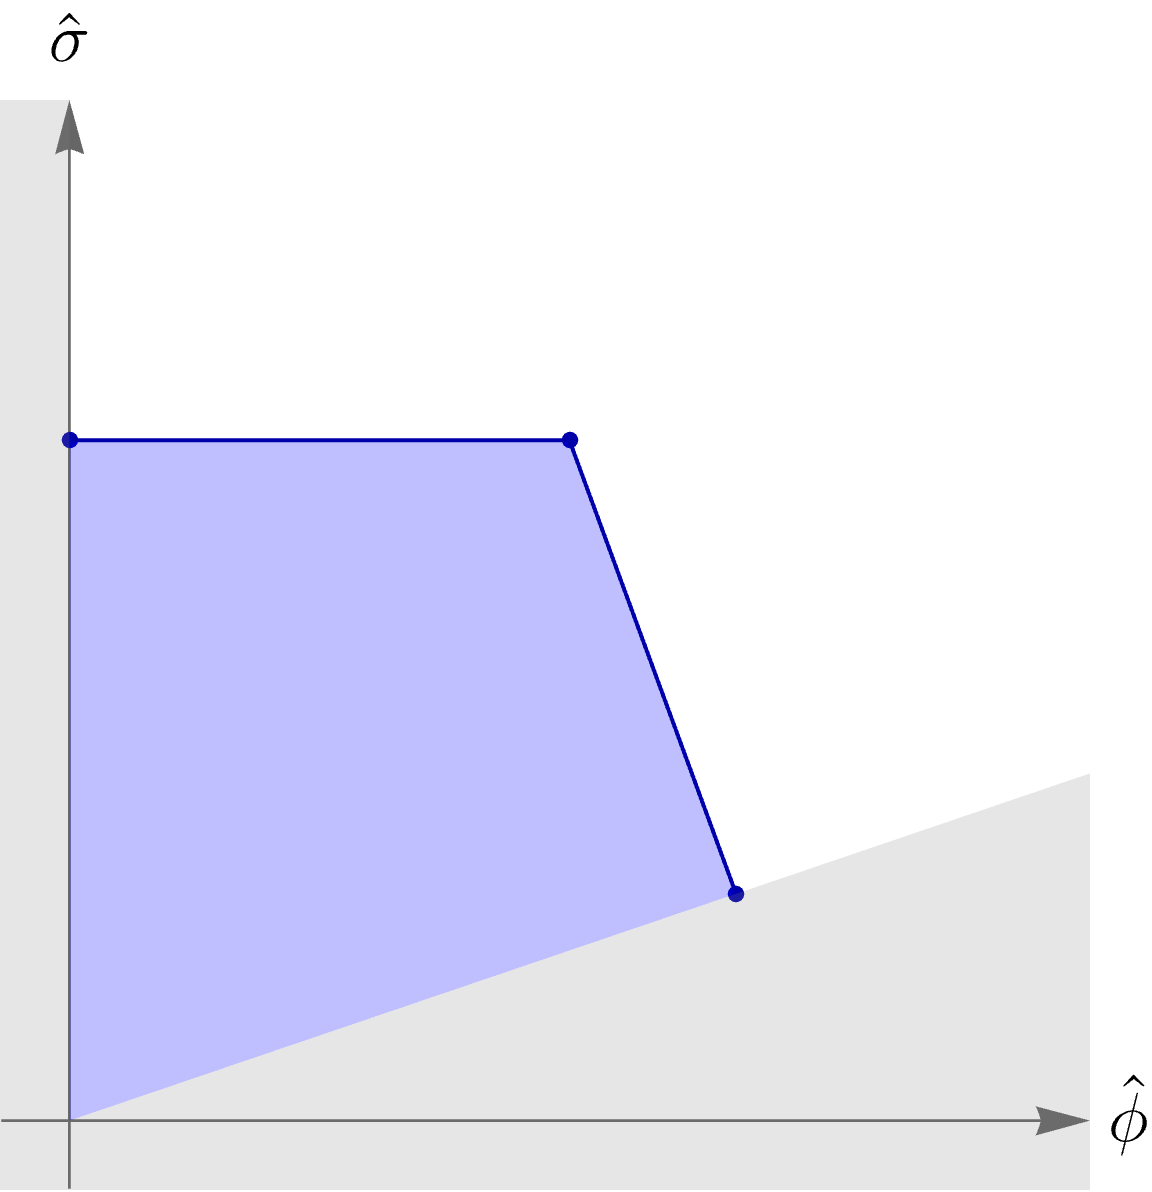
\includegraphics[width=0.45\textwidth]{CH-example.png}
\caption{\small Example of the convex hull generated by the triplet of vectors in \eqref{vectors}, restricted to the region in which the towers of states are enough to build it. In the region shaded in grey, new towers potentially arising from extended objects in $D$-dimensions are expected to become relevant and complete the rest of the diagram.} 
\label{fig:ch-example}
\end{center}
\end{figure}
%%%%%%%%%%%%

Let us start with the first boundary, namely the edge joining $\vec{\mathcal{Z}}_{\text{KK}}$ with $\vec{\mathcal{Z}}_{\text{KK-t},\, p+1}$. As one can clearly see, this line is horizontal for any value of $\lambda_{\text{sp}}$ and $p$. Furthermore, the distance from this edge to the origin is always given by the saturating value
%
\begin{equation}\label{eq:lspmin}
    \lambda_{\text{sp}, \, \text{min}}\, =\, \frac {1}{\sqrt{(d-1)(d-2)}} \, ,
\end{equation}
%
again irrespective of the values of $\lambda_{\text{sp}}$ and $p$. Therefore, we conclude that \eqref{eq:lowerboundspecies2} is indeed the \emph{strongest} possible bound yet compatible with dimensional reduction on a circle (see also the discussion after eq. \eqref{eq:Zspeciescompactification}). The fact that the KK tower associated to some internal $\mathbf{S}^1$ typically yields this particular value was pointed out as well in \cite{vandeHeisteeg:2023uxj} as a bottom-up argument for the latter. Moreover, their results regarding the global behaviour of the species cut-off in 4d $\mathcal{N}=2$ theories suggest that \eqref{eq:lowerboundspecies2} could be extended slightly beyond the strictly asymptotic regime, due to the positivity of the generic leading-order logarithmic corrections found therein. Here we also uncover that, if the $(d+1)$-dimensional theory has some non-trivial moduli space, it is crucial to take into account the effective towers for the CHC to be satisfied in the lower-dimensional EFT. In particular, the saturation featured by the vector $\vec{\mathcal{Z}}_{\text{KK}}$ towards the $\hat \sigma \to \infty$ limit would actually present a pressing problem for the bound to be satisfied along other neighbouring directions, unless some additional species vectors were present. These must be, in addition, tightly constrained, since otherwise the resulting convex hull would not contain the ball of radius $\frac {1}{\sqrt{(d-1)(d-2)}}$. Fortunately, we are able to find a vector --- namely $\vec{\mathcal{Z}}_{\text{KK-t},\, p+1}$ --- that precisely accomplishes this, regardless of the details of the tower already existing in $D$-dimensions. Let us also stress that, since we interpret $\hat \phi$ as parametrizing any geodesic trajectory in the moduli space of the parent $D$-dimensional theory, the above conclusion is in fact not limited to theories with just one single field. %In summary, we find a pretty robust mechanism protecting the CHC for the $\lambda_{\rm sp}$--\,parameter condition whenever saturation is attained by means of some KK tower associated to one extra dimension.

For the remaining boundary, namely the line determined by the vectors $\vec{\mathcal{Z}}_{\text{KK-t},\, p+1}$ and $\vec{\mathcal{Z}}_{\text{t}}$, we first note that at fixed $\lambda_{\text{sp}}$, varying $p$ only modifies the length of the corresponding edge but not its slope. This means, in practice, that the distance from the origin to this facet of the polytope is bounded from below by that associated to its infinite length extension. Second, we realize that $\lambda_{\text{sp}}$ only appears in the first components of the vectors \eqref{vectors}, and it does so in such a way that the bigger $\lambda_{\text{sp}}$, the farther away from the origin this edge will appear. In physical terms, this means that the closer we are to violate \eqref{eq:lowerboundspecies2} in $D$-dimensions, the easier it gets to do so after dimensional reduction as well. As a consequence, we deduce that the most dangerous situation happens precisely when the bound is saturated in the higher-dimensional theory. Nevertheless, even in this scenario there is no violation whatsoever of the CHC, regardless of the particular value of $p$ (see Figure \ref{fig:dim-red}), and in fact one finds again saturation when $p=1$. %Let us however notice that, even though in this general approach we let $p$ take any value, having $p<1$ seems rather unphysical from our experience with string theory examples.

%%%%%%%%%%%%
\begin{figure}[htb]
\begin{center}
	\subfigure[\label{sfig:4dp=0.2}$d=4$ and $p=0.2$]{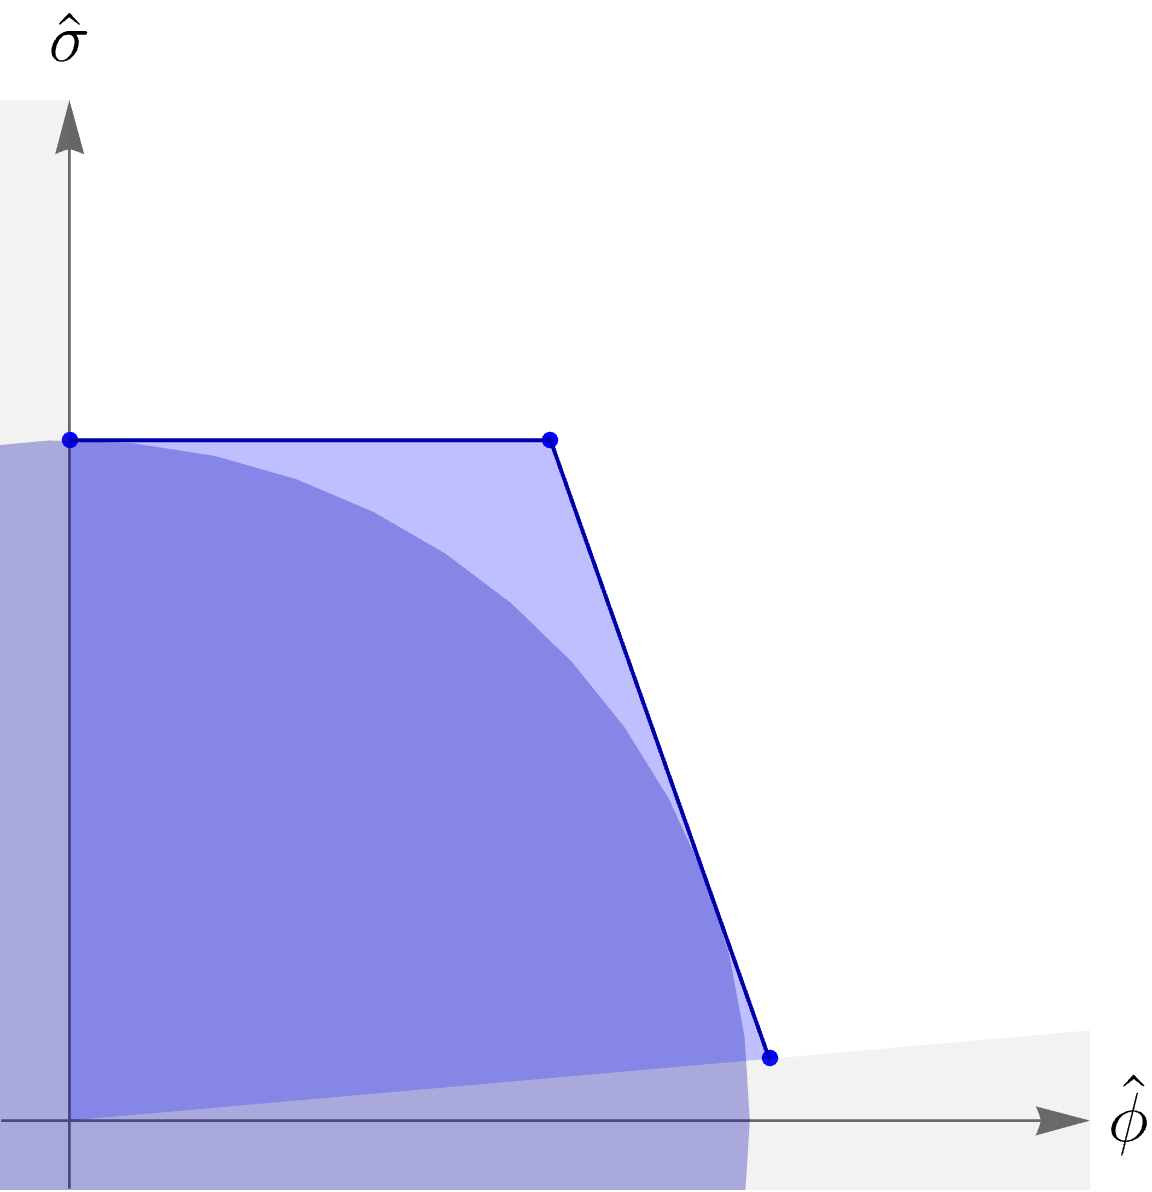
\includegraphics[width=0.32\textwidth]{dim-red-1.png}}
	\subfigure[\label{sfig:4dp=1}$d=4$ and $p=1$]{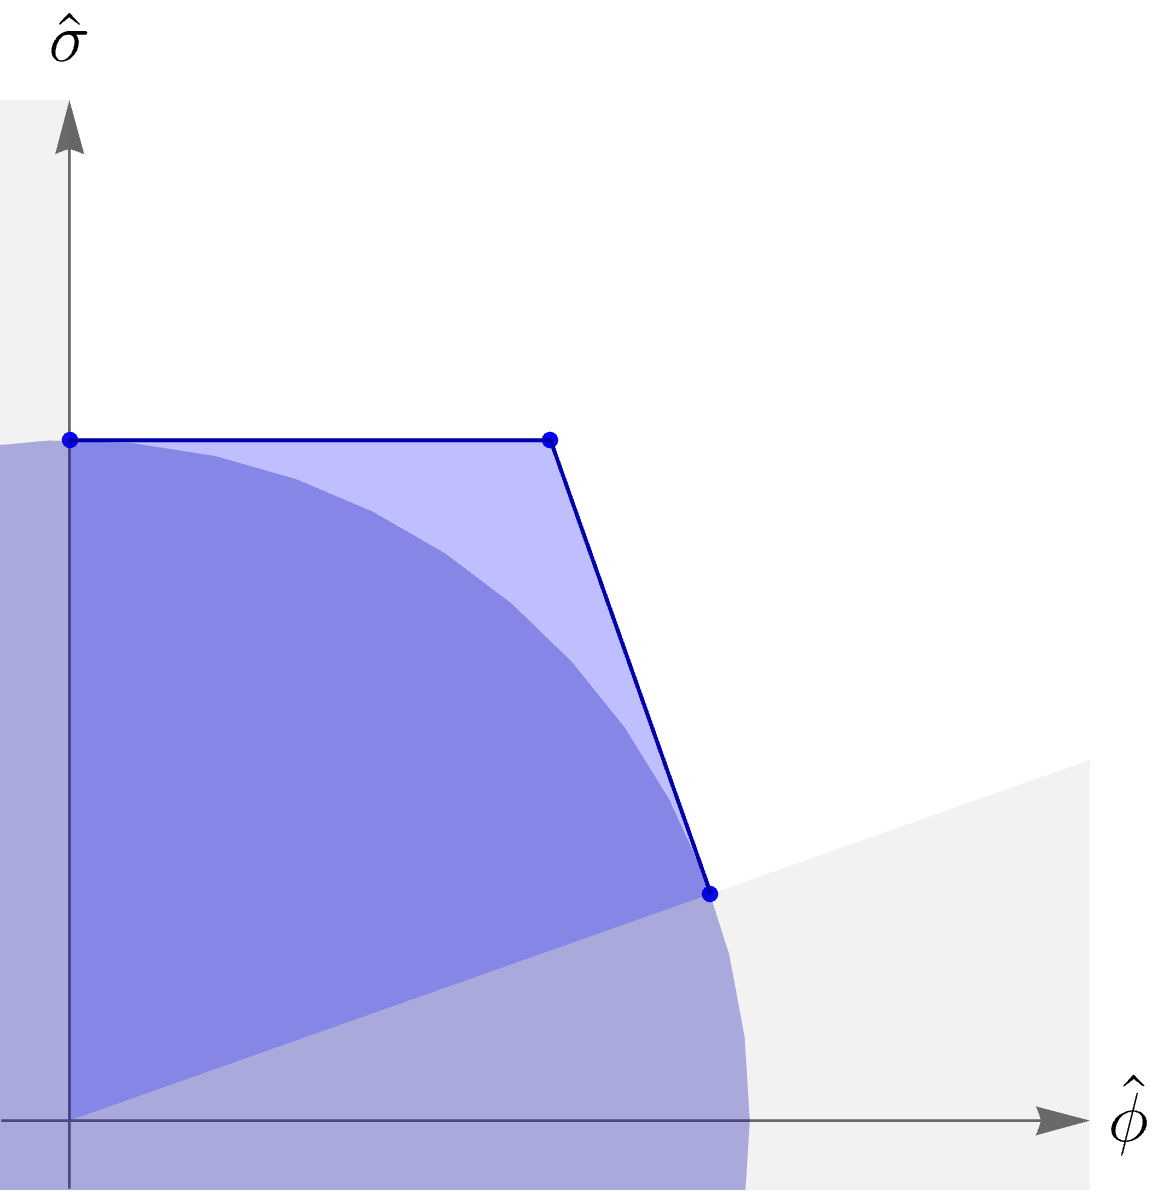
\includegraphics[width=0.32\textwidth]{dim-red-2.png}}
	\subfigure[\label{sfig:4dp=5}$d=4$ and $p=5$]{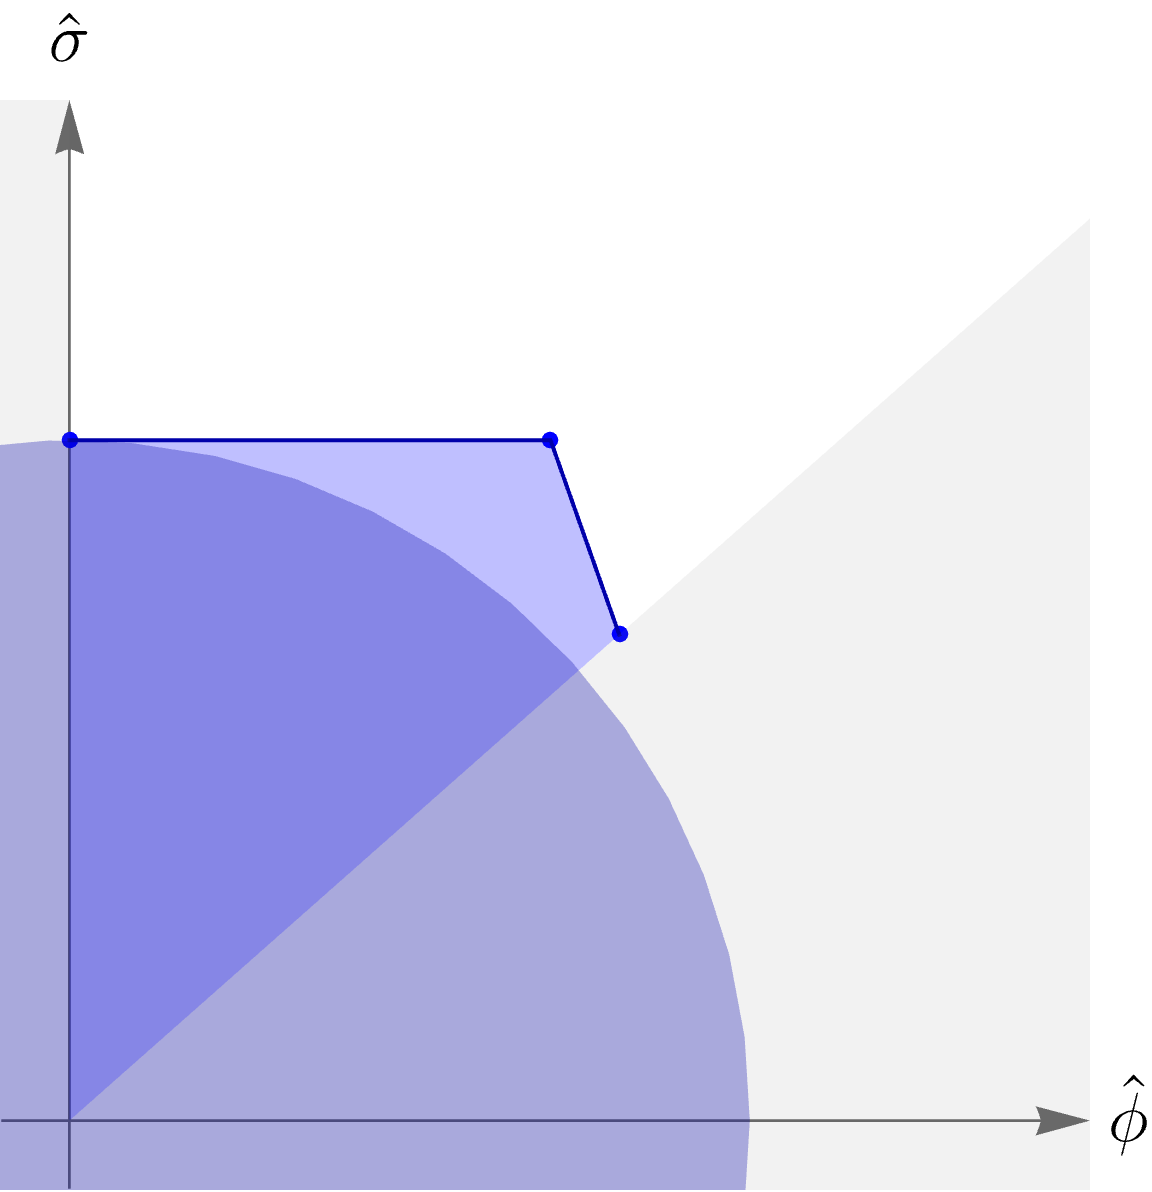
\includegraphics[width=0.32\textwidth]{dim-red-3.png}}
	\caption{Convex hull diagrams for the species scale vectors in four dimensions. We assume that the parent 5-dimensional theory is such that $\lambda_{\text{sp}}$ saturates \eqref{eq:lowerboundspecies2}, and show the resulting plot for three different values of $p$.}
	\label{fig:dim-red}	
\end{center}
\end{figure}
%%%%%%%%%%%%

In conclusion, we see that the bound \eqref{eq:lowerboundspecies2} is preserved under dimensional reduction on a circle, at least for those asymptotic directions where field-theoretic considerations suffice to determine the convex hull diagram. In fact, it can be regarded as the strongest bound on the exponential decay rate of the species scale yet compatible with this procedure. This moreover involves a pretty robust mechanism, where the CHC is crucially protected by the KK replicas of the tower already existing in the higher-dimensional theory. 

\subsubsection*{Generalization to $D=d+n$ dimensions}

It is worth emphasizing that the previous analysis also extends to the more general case of compactification on a $n$-dimensional Ricci-flat manifold $\mathcal{X}_n$ (e.g., a $\mathbf{T}^n$). To see this, we start by reducing the original $D$-dimensional EFT on $\mathcal{X}_n$, such that the relevant dynamics in $d$ dimensions is described by the action (see Appendix \ref{ap:generalities} for details)
%
\begin{equation}
	S_{d} \supset \int \dd^{d}x\, \sqrt{-g}\,  \left[ \frac{1}{2\kappa_{d}^2} \left(\mathcal{R} - \frac{d+n-2}{n (d-2)} \left(\partial \log \mathcal{V}_n \right)^2 \right)- \frac{1}{2} \left(\partial \hat \phi \right)^2 \right]\, ,
\end{equation}
%
where $\mathcal{V}_n$ denotes the overall volume modulus measured in $D$-dimensional Planck units and we have retained only the massless scalar-tensor sector of the theory. Hence, upon canonically normalizing the volume modulus
%
\begin{equation}
	\hat \sigma = \frac{1}{\kappa_d}\sqrt{\frac{d+n-2}{n(d-2)}} \log \mathcal{V}_n\, ,
\end{equation}
%
one finds again two competing scalar charge-to-mass vectors, namely the one associated to the isotropic KK tower (with density parameter $p_{\text{KK}}=n$) and the original $D$-dimensional tower, which read
%
\begin{equation}\label{eq:zvectornmfd}
	\vec{\zeta}_{\text{KK},\, n} = \left( 0 \ ,\ \sqrt{\frac{d+n-2}{n(d-2)}} \right) \, , \quad \vec{\zeta}_{\text{t}} = \left( \lambda_{\text{t}} \ ,\ \sqrt{\frac{n}{(d+n-2)(d-2)}} \right) \, .
\end{equation}
%
From these one obtains three species vectors
%
\begin{equation}
\label{eq:Zspeciescompactification}
\begin{split} 
	&\vec{\mathcal{Z}}_{\text{KK},\, n} = \left( 0 \ ,\ \sqrt{\frac{n}{(d+n-2)(d-2)}} \right) \, ,\\
	&\vec{\mathcal{Z}}_{\text{t}} = \left( \frac{d-1+p}{d-2+p} \ \lambda_{\text{sp}} \ ,\ \frac{p}{d-2+p} \sqrt{\frac{n}{(d+n-2)(d-2)}} \right) \, ,\\
	&\vec{\mathcal{Z}}_{\text{KK-t},\, p+n}  = \left( \frac{d-1+p}{d-2+n+p} \ \lambda_{\text{sp}} \ ,\ \sqrt{\frac{n}{(d+n-2)(d-2)}} \right) \, .
\end{split}
\end{equation}
%
Notice that, as in the previous $\mathbf{S}^1$--\,compactification, we see that the boundary of the convex hull determined by $\vec{\mathcal{Z}}_{\text{KK},\, n}$ and $\vec{\mathcal{Z}}_{\text{KK-t},\, p+n}$ is again horizontal. Strictly speaking, though, this is not needed anymore so as to protect the CHC, since $\vec{\mathcal{Z}}_{\text{KK},\, n}$ does actually satisfy the bound with room to spare when $n>1$. In any event, the conclusion remains unchanged, thus confirming the expectation that the most constraining compactification for the exponential rate of the species scale corresponds to $n=1$, i.e. a circle/interval reduction.

Similarly, it is straightforward to check that the slope of the edge connecting $\vec{\mathcal{Z}}_{t}$ and $\vec{\mathcal{Z}}_{\text{KK-t},\, p+n}$ is also independent of $p$. Moreover, the larger $\lambda_{\text{sp}}$ the farther away from the origin that the corresponding edge gets. In fact, in the most dangerous situation, i.e. when \eqref{eq:lowerboundspecies2} is saturated in $D=d+n$ dimensions, this line still preserves the CHC in the lower dimensional theory, leading again to saturation if $p = 1$. %The convex hull in this case looks very much the same like the ones in Figure \ref{fig:dim-red}, but with the upper edge being shifted above according to the second component of $\vec{\mathcal{Z}}_{\text{KK},\, n}$ while keeping fixed that the infinite length extension of the other line touches the ball. 
All in all, the claim that the bound \eqref{eq:lowerboundspecies2} is preserved under dimensional reduction (within the directions in which field theory is enough to determine the convex hull), remains true for $n>1$ compactifications as well.    

\subsection{Beyond field theory}
\label{ss:compactificationstring}

The aim of this subsection is to go beyond our previous field-theoretical considerations and study the fate of the bound \eqref{eq:lowerboundspecies2} after the inclusion of genuine quantum-gravitational ingredients. To illustrate this, we consider a very simple toy model which is clearly inspired by Type IIB string theory, thus featuring two fundamental strings in $D$ spacetime dimensions. These strings may become asymptotically tensionless when exploring two different infinite distance regimes. For simplicity, we will again restrict ourselves to one-dimensional moduli spaces, where the previous emergent string limits arise upon taking $\hat \phi \to \pm \infty$. Therefore, we assume the associated string excitation modes to become exponentially massless with some constant decay rate $\lambda_{\text{osc}}$ (correspondingly $\lambda_{\text{osc}'} =-\lambda_{\text{osc}}$), which in this case coincides with the exponential rate for the species scale. 

The dimensional reduction analysis of the aforementioned theory on a circle proceeds exactly as in Section \ref{ss:field-theory}, with the important difference that we can have additional towers in $d$ dimensions arising from the winding modes of the extended strings. The relevant scalar charge-to-mass vectors read \cite{Etheredge:2022opl}
%
\begin{equation}\label{eq:zvectorsp=1}
\begin{split} 
	\vec{\zeta}_{\text{KK}} =& \left( 0 \ ,\ \sqrt{\frac{d-1}{d-2}} \right)\, , \qquad \vec{\zeta}_{\text{w}} = \left( 2 \lambda_{\text{osc}} \ ,\ - \frac{d-3}{\sqrt{(d-1)(d-2)}} \right) \, ,\\
	\vec{\zeta}_{\text{w}'} =& \left( -2 \lambda_{\text{osc}} \ ,\ - \frac{d-3}{\sqrt{(d-1)(d-2)}} \right) \, ,
\end{split}
\end{equation}
%
for the KK-like towers, whilst for the string oscillator modes one rather finds
%
\begin{equation}\label{eq:zvectorsStrings}
  \vec{\zeta}_{\text{osc}} =\left( \lambda_{\text{osc}} \ ,\ \frac{1}{\sqrt{(d-1)(d-2)}} \right) \, , \qquad 
  \vec{\zeta}_{\text{osc}'} = \left( - \lambda_{\text{osc}} \ ,\ \frac{1}{\sqrt{(d-1)(d-2)}} \right) \, .
\end{equation}
%
Moreover, upon using eq. \eqref{eq:eff-vector} above, we can translate the set \eqref{eq:zvectorsp=1} into the following species scale vectors
%
\begin{equation}\label{vectors2}
\begin{split} 
	\vec{\mathcal{Z}}_{\text{KK}} =& \left( 0 , \frac{1}{\sqrt{(d-1)(d-2)}} \right)\, , \qquad \qquad \qquad \ \ \vec{\mathcal{Z}}_{\text{w}} = \left( \frac{2 \lambda_{\text{osc}}}{d-1} , - \frac{d-3}{(d-1)^{3/2}\sqrt{(d-2)}} \right) \, ,\\
	\vec{\mathcal{Z}}_{\text{w}'} =& \left( -\frac{2 \lambda_{\text{osc}}}{d-1} , - \frac{d-3}{(d-1)^{3/2}\sqrt{(d-2)}} \right) \, , \quad \vec{\mathcal{Z}}_{\text{w}, \,2} = \left( 0 , - \frac{2(d-3)}{d\sqrt{(d-1)(d-2)}} \right) \, .
\end{split}
\end{equation}
%
Here we have taken into account several things. First, notice that even though strings can form effective towers together with some additional KK-like spectrum, their degeneracy is so strong that they already dominate the state counting and thus saturate the species scale alone.\footnote{Recall that this claim can be intuitively understood upon taking $p\to\infty$ in eq. \eqref{eq:eff-vector}, which forces the species scale to be given precisely by the fundamental string scale.} Additionally, we have assumed the two towers of winding modes to be multiplicative, thus giving rise to the effective species vector $\vec{\mathcal{Z}}_{\text{w}, \,2}$, which has $p=2$. In Type IIB string theory this comes about from having not only the fundamental and the D1-string, but also the spectrum of $(p,q)$ bound states thereof \cite{Witten:1995im}. We will see later on how this fits nicely with the results. Finally, in spite of the fact that one could also a priori consider winding and KK modes to be multiplicative amongst each other, their effective combination ends up being, to all effects, irrelevant for testing the CHC, as one may readily check.

With this information, we are now ready to study the behavior of the bound \eqref{eq:lowerboundspecies2} under dimensional reduction within the present toy model. As a first interesting observation, let us note that $\lambda_{\text{osc}}$ only appears in the first components of (some of) the vectors in eqs. \eqref{eq:zvectorsStrings} and \eqref{vectors2}, in such a way that for larger values of $\lambda_{\text{osc}}$, these vectors get farther away from the origin, similarly to what happened in Section \ref{ss:field-theory}. Following the same logic as in there, one can then try to fix $\lambda_{\text{osc}}$ so as to saturate the CHC in the parent $D$-dimensional theory, namely
%
\begin{equation}
    \lambda_{\text{osc}} \stackrel{!}{=} \frac{1}{\sqrt{(D-1)(D-2)}} = \frac{1}{\sqrt{d(d-1)}} \, .
\end{equation}
%
Plugging this into the previous set of $\mathcal{Z}$-vectors and drawing the convex hull, one realizes that there seems to be an unavoidable violation of the bound \eqref{eq:lowerboundspecies2} for any spacetime dimension $d$. (An example of this is shown in Figure \ref{fig:ch3} for the $d=9$ case.) Let us stress, however, that this by itself does \emph{not} imply a violation of the CHC for the species scale within quantum gravity in general, since we are just considering a very crude toy model in which there exists some critical string with decay rate $\lambda_{\text{osc}}$ that is moreover taken to saturate \eqref{eq:lowerboundspecies2} in $D$-dimensions. In fact, as we know from our experience with string theory, critical strings never feature this particular value for the exponential decay rate along their own gradient flow, but instead a much \emph{larger} one. In a sense, what this toy model tells us is that the consistency of the CHC prevents the strings from saturating alone the lower bound \eqref{eq:lowerboundspecies2}. This resembles prior studies in the literature of certain Swampland criteria, which under some circumstances become stronger when imposing its consistency under dimensional reduction (see e.g., \cite{Heidenreich:2015nta}).

%%%%%%%%%%%%
\begin{figure}[htb]
\begin{center}
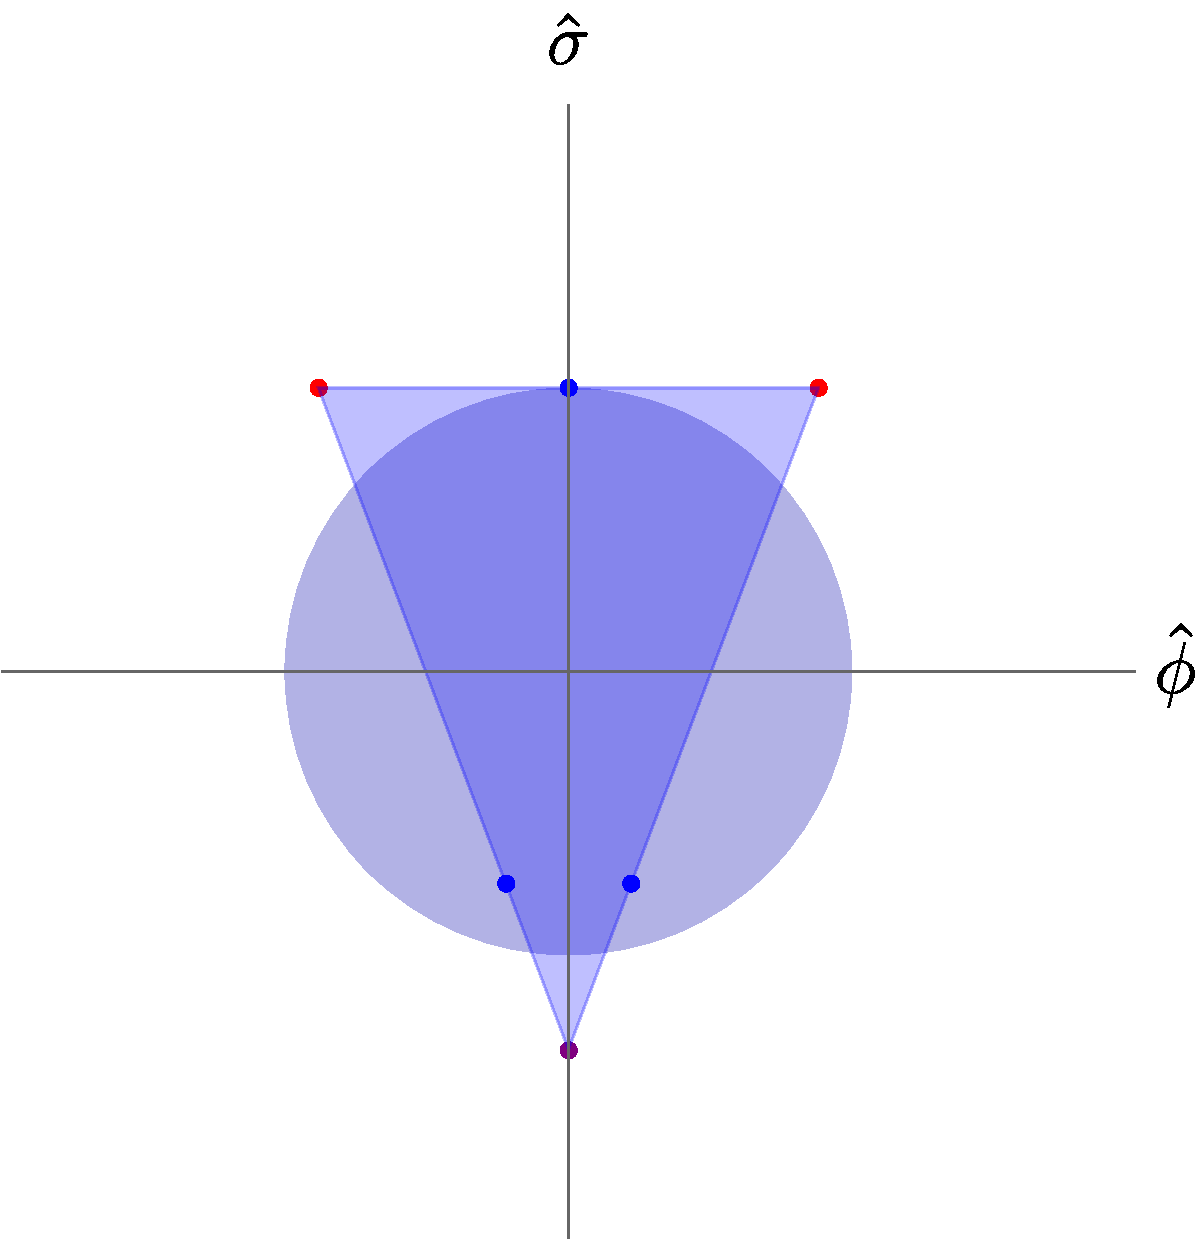
\includegraphics[width=0.45\textwidth]{CH-3.pdf}
\caption{\small Convex hull diagram for a theory featuring two fundamental strings (red dots) that saturate the CHC \eqref{eq:lowerboundspecies2} in $D=10$ dimensions, after compactification on $\mathbf{S}^1$. The blue dots are associated to KK-like towers with $p=1$, whilst the purple one represents the effective winding tower of $p=2$. Finally, the axes correspond to the radius modulus $\hat \sigma$ as well as the $D$-dimensional dilaton, $\hat \phi$.} 
\label{fig:ch3}
\end{center}
\end{figure}
%%%%%%%%%%%%

Therefore, following our discussion in the previous paragraph, a better justified value for $\lambda_{\text{osc}}$ would be (c.f. eq. \eqref{eq:zetaveconemodulus})
%
\begin{equation}
    \lambda_{\text{osc}} = \frac{1}{\sqrt{D-2}} = \frac{1}{\sqrt{d-1}} \, .
\end{equation}
%
After plugging this into eqs. \eqref{eq:zvectorsStrings} and \eqref{vectors2} so as to draw the convex hull, we find that the CHC is a priori satisfied only for $D \geq 10$, see Figure \ref{fig:ch4} for the particular cases of $D=5$ and $D=9$. Furthermore, we find saturation happening precisely in the ten-dimensional case. %Indeed, notice that, as shown in Figure \ref{fig:ch5}, this latter case precisely recovers a rotated version of the convex hull depicted in Figure \ref{fig:ch1} above. 
Of course, this is not a coincidence, since in this case our toy model precisely reproduces Type IIB string theory on $\mathbf{S}^1$, which is known to be dual to M-theory on $\mathbf{T}^2$, see Section \ref{ss:MthyT2SSDC} below.

%%%%%%%%%%%%
\begin{figure}[htb]
\begin{center}
	\subfigure[\label{sfig:5dto4d}$D=5 \, \rightarrow\, d=4$]{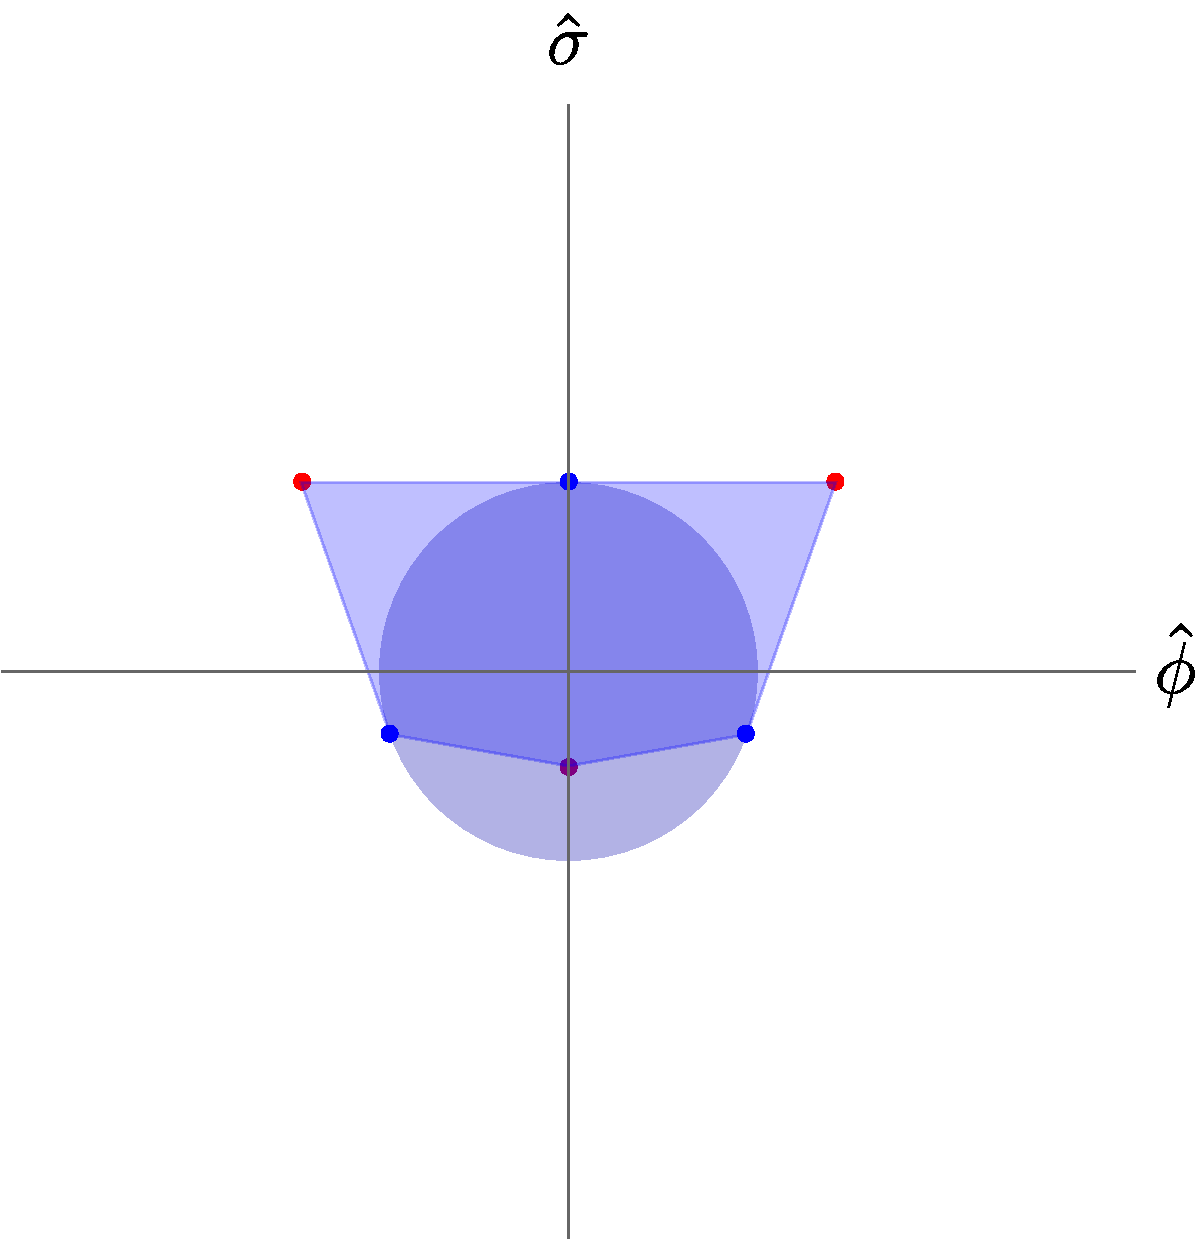
\includegraphics[width=0.45\textwidth]{CH-4.pdf}}\qquad 
	\subfigure[\label{sfig:9dto8d}$D=9 \, \rightarrow\, d=8$]{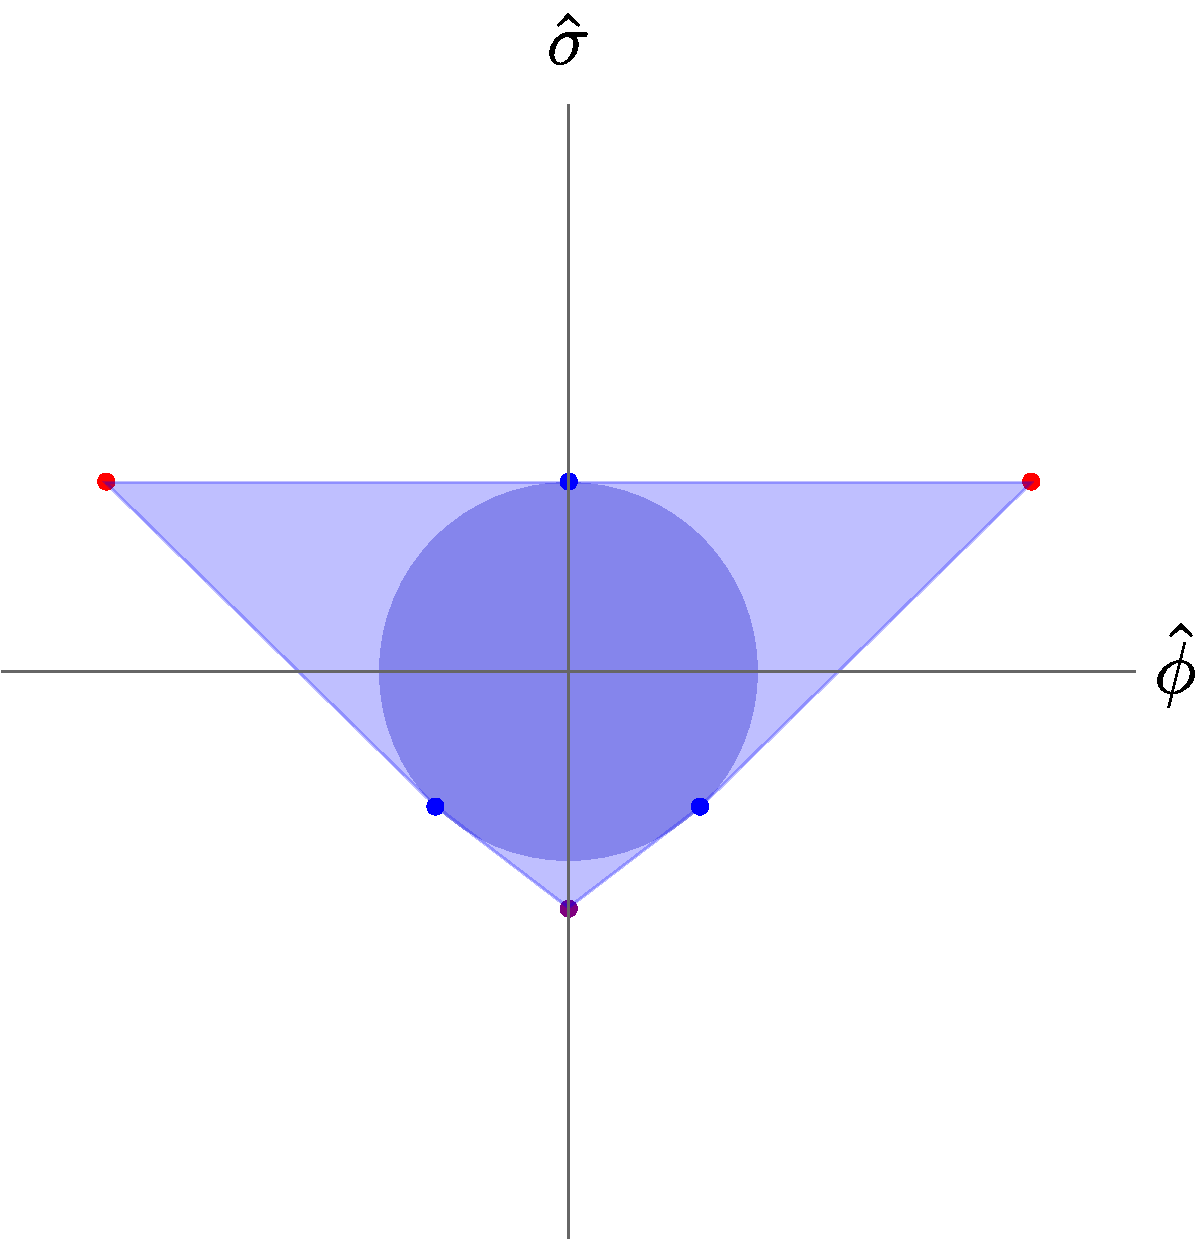
\includegraphics[width=0.45\textwidth]{CH-5.pdf}}
	\caption{Convex hull diagram of a theory of strings with $|\lambda_{\rm osc}|=\frac{1}{\sqrt{D-2}}$ in \textbf{(a)} $D=5$ and \textbf{(b)} $D=9$ dimensions compactified on a circle. Although difficult to spot by eye, one may easily check that the 9d $\to$ 8d case also violates the CHC for asymptotic directions centered around the two lower blue dots, corresponding to T-dual decompactifications of one extra dimension.}
	\label{fig:ch4}	
\end{center}
\end{figure}
%%%%%%%%%%%%

%%%%%%%%%%%%
\begin{figure}[htb]
\begin{center}
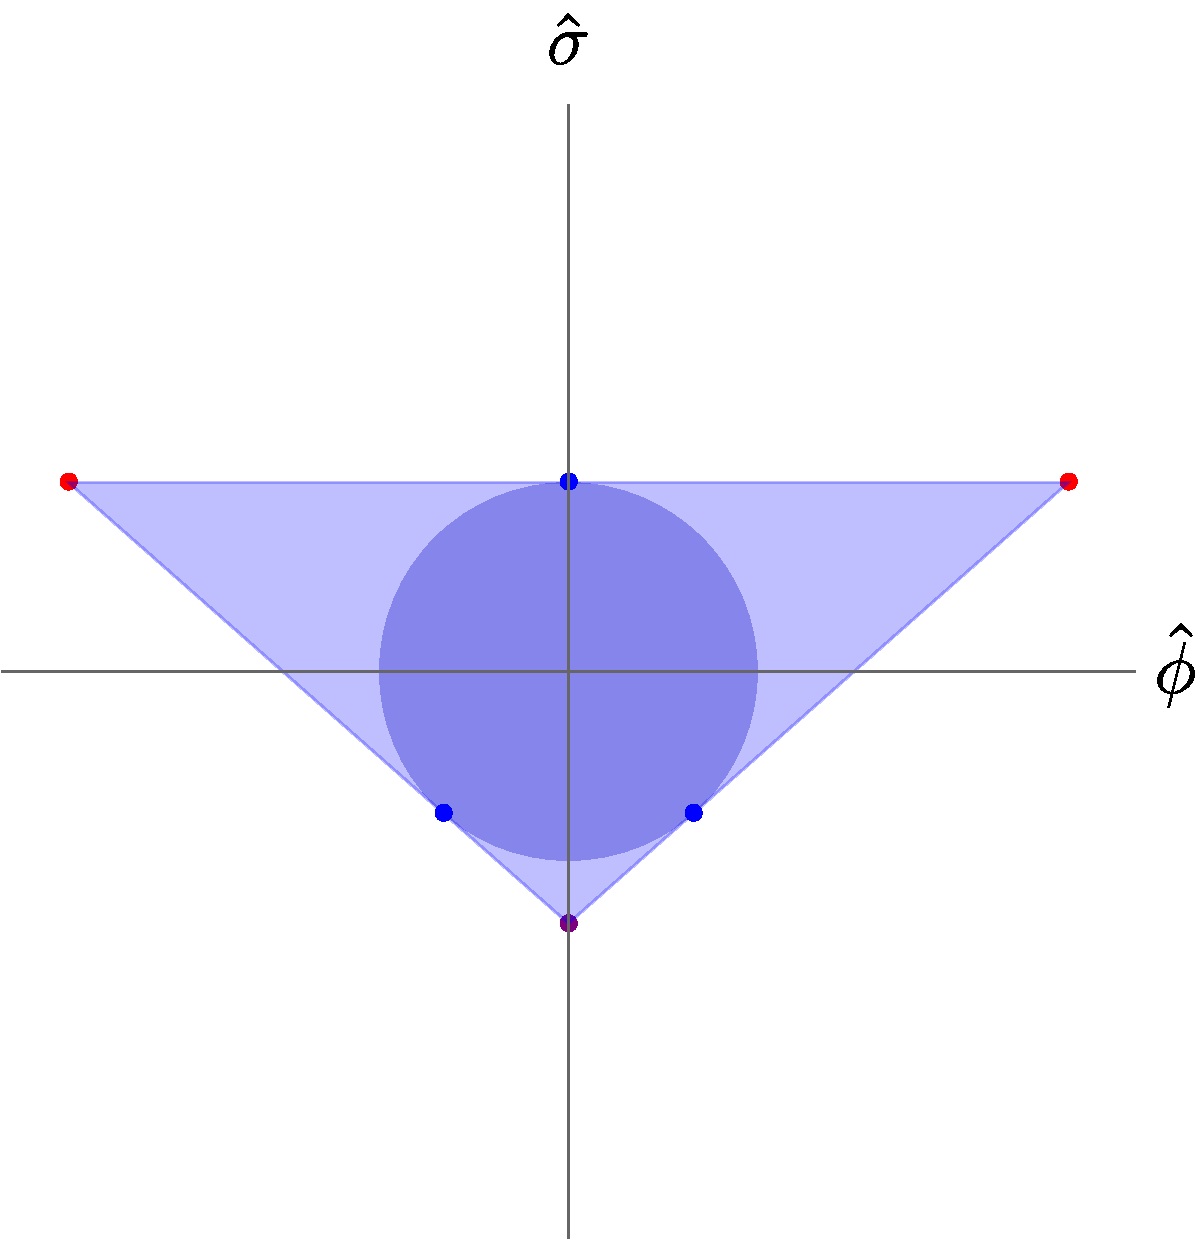
\includegraphics[width=0.45\textwidth]{CH-6.pdf}
\caption{\small Convex hull diagram of a theory of strings with $|\lambda_{\rm osc}|=\frac{1}{\sqrt{D-2}}$ in $D=10$ dimensions compactified on a circle. It can be related with the corresponding picture in M-theory on $\mathbf{T}^2$ after a $\pi/2$ rotation, c.f. Figure \ref{fig:ch1}.} 
\label{fig:ch5}
\end{center}
\end{figure}
%%%%%%%%%%%%

Very remarkably, we conclude that the present toy model, which presents only one-dimensional strings to start with, does not satisfy the bound \eqref{eq:lowerboundspecies2} in $D\leq 9$ after dimensionally reducing on a circle. This is actually consistent with our intuition from string theory, since upon compactifying down to $d\leq8$ dimensions, not only strings and winding modes arise, but also higher-dimensional non-perturbative objects do, such as D$p$-branes. Such extended objects potentially give rise --- when wrapped along some internal cycle of the compact geometry --- to new infinite towers of states. Indeed, an explicit realization of these matters will be presented later on in Section \ref{ss:MthyT3SSDC}, where we consider M-theory compactified on $\mathbf{T}^3$. There, we will not only verify the CHC but we will also be able to construct a picture that is very reminiscent of the one shown in Figure \ref{sfig:9dto8d}, which features certain additional towers that indeed protect the lower bound \eqref{eq:lowerboundspecies2} in a non-trivial manner.

Before closing this subsection, let us compare our results with the ones obtained for the sharpened Distance Conjecture \cite{Etheredge:2022opl}. There it was shown, by considering the exact same toy model, that the winding modes associated to the critical strings were in fact sufficient so as to ensure that the bound \eqref{eq:sharpenedDistConj} holds in $d\geq5$. Additionally, it was argued that a tower of KK monopoles prevents this condition from being violated in $d=4$. Here we find that the analogous condition for the species scale decay rate requires from more than this. Indeed, as argued before, the presence of higher-dimensional objects in $D$-dimensions seems to be crucial for the CHC to be satisfied in lower dimensional (Minkowski) vacua as soon as we get down to nine non-compact dimensions. %Again, it turns out that under some circumstances, the SSDC becomes more powerful after imposing its consistency under dimensional reduction. 

\section{String theory evidence}
\label{s:examplesbound}

In this section we present non-trivial evidence in favour of the proposed lower bound for the asymptotic decay rate of the species scale in theories of quantum gravity. We will restrict ourselves to maximally supersymmetric set-ups arising from toroidal compactifications of Type II/M-theory, where the verification of \eqref{eq:lowerboundspecies2} becomes highly intricate even in the most simple cases. In particular, in Sections \ref{ss:MthyT2SSDC} and \ref{ss:MthyT3SSDC} we study the problem very explicitly in maximal supergravity in nine and eight spacetime dimensions. Later on, in Section \ref{ss:MthyTk}, we present a brief argument extending the proof to lower-dimensional toroidal compactifications as well. For completeness, let us mention that the convex hull diagrams here presented can be regarded as `boundary conditions' that any globally defined species scale function must agree with, see Chapter \ref{ch:Higherdimops} for details on this. 

\subsection{M-theory on $\mathbf{T}^2$}
\label{ss:MthyT2SSDC}

We consider first a 9d $\mathcal{N}=2$ example arising from compactifying M-theory on a two-dimensional torus. The bosonic action for the scalar and gravitational sectors reads
%
\begin{equation}\label{eq:9d}
	S^{\text{9d}}_{\text{M-th}} \supset \frac{1}{2\kappa_9^2} \int \dd^{9}x\, \sqrt{-g}\,  \left( \mathcal{R} - \frac{9}{14} \left( \frac{\partial \mathcal{V}_2}{\mathcal{V}_2} \right)^2 -\frac{\partial \tau \cdot \partial \bar \tau}{2 \left(\text{Im}\, \tau\right)^2} \right)\, ,
\end{equation}
%
where $\tau=\tau_1+ \i \tau_2$ and $\mathcal{V}_2$ are the complex structure and the volume of the $\mathbf{T}^2$, respectively (see Section \ref{ss:9dmaxsugra} for details). As discussed in Section \ref{s:dualities}, this theory enjoys a non-perturbative $\mathsf{SL(2, \mathbb{Z})}$ duality symmetry, whose origin is clearly geometric from this perspective since it is associated to the group of large diffeomorphisms of the internal torus\cite{Schwarz:1995dk,Aspinwall:1995fw}. 

Our goal here will be to check the convex hull condition for the species scale, namely the requirement
%
\begin{equation} \label{eq:bound9d}
  \lambda_{\text{sp}} \geq \frac{1}{\sqrt{(d-1)(d-2)}} \stackrel{\text{9d}}{=} \frac{1}{\sqrt{56}}\, ,
\end{equation}
%
at any boundary of moduli space. Moreover, since this condition should hold for any locally geodesic trajectory within the latter as it explores infinite distance, the first step is to properly characterize the latter. For this, we recall that the 9d moduli space can be identified with group coset
%
\begin{equation}\label{eq:9dmodspaceSSDC}
 \mathcal{M}_{\text{9d}}=\mathsf{SL(2, \mathbb{Z})}\backslash \mathsf{SL(2, \mathbb{R})}/\mathsf{U(1)} \times \mathbb{R}_+\, ,
\end{equation}
%
where we have already modded out by the modular duality group. Furthermore, as we discuss in more detail below, all geodesic trajectories reaching infinity are such that $\tau_1 \to \text{const.}$ asymptotically. This allows us to restrict our discussion to the slice of $\mathcal{M}_{\text{9d}}$ parametrized by the non-compact directions $\{ \mathcal{V}_2, \text{Im}\, \tau \}$, which corresponds to the subspace of asymptotically geodesic tangent vectors introduced in ref. \cite{Calderon-Infante:2020dhm}.

In a next step, one needs to account for the relevant towers of states, as well as compute all possible quantum gravity cut-offs that could arise depending on the infinite distance singularity that we probe. We start by considering $\frac{1}{2}$-BPS strings, which arise from wrapped M2-branes on any $(p,q)$ 1-cycle of the internal geometry. Their tension can be computed to be
%
\begin{equation}\label{eq:pqstrings9d}
	T_{p,q} = \frac{2\pi}{\ell_{9}^2} \frac{|p+q\tau|}{\sqrt{\tau_2}} \mathcal{V}_2^{\frac{3}{14}}\, ,
\end{equation}
%
where $\ell_{9}$ denotes the 9d Planck length. In the following, we will fix the axion v.e.v. to zero for simplicity (see however the discussion after eq. \eqref{eq:chargetomasspq}), and only keep track of the saxionic dependence of the relevant masses involved. We moreover define canonically normalized fields $\hat U$ and $\hat \tau$ as follows
%
\begin{equation} \label{eq:canonicalnormalization}
  \log \mathcal{V}_2 =  \kappa_9 \sqrt{\frac{14}{9}}\, \hat U \, , \quad \tau_2 = \kappa_9\, e^{\sqrt{2} \, \hat\tau} \, ,
\end{equation}
%
in terms of which the mass scale of the oscillation modes of the $(p,q)$-strings reads as
%
\begin{equation} \label{strings}
  m^{(\text{osc})}_{p,q} = \sqrt{T_{p,q}} =  \frac{(4\pi)^{5/14} M_{\text{Pl};\, 9}}{\sqrt{2}} \left( p^2 e^{-\sqrt{2} \,\hat\tau} + q^2 e^{\sqrt{2} \,\hat\tau}\right)^{1/4} e^{\frac{1}{2 \sqrt{14}} \, \hat U} \, .
\end{equation}
%
Note that the above expression presents two different asymptotic behaviors depending on which infinite distance limit is probed and whether $p$ and $q$ are non-vanishing. As it is to be expected, any infinite distance limit --- at fixed $\tau_1=0$ --- is dominated by either the $q=0$ or $p=0$ cases, which are associated to the fundamental and S-dual Type II strings, respectively. These lead to two relevant asymptotic scales for the QG cut-off
%
\begin{equation} \label{string-species}
  \frac{\Lambda_{\text{osc}}}{M_{\text{Pl};\, 9}}\, \sim\, e^{\frac{1}{2 \sqrt{14}} \, \hat U-\frac{1}{2\sqrt{2}} \,\hat\tau } \, , \qquad \frac{\Lambda_{\text{osc'}}}{M_{\text{Pl};\, 9}}\, \sim\, e^{\frac{1}{2 \sqrt{14}} \, \hat U + \frac{1}{2\sqrt{2}} \,\hat\tau } \, ,
\end{equation}
%
where we are using the fact that the species scale associated to a critical string is given at leading order by its own mass. One thus obtains the following relevant species vectors
%
\begin{equation}
\label{eq:speciesscalevectorsstringsT2}
  \vec{\mathcal{Z}}_{\text{osc}} = \left( -\frac{1}{2 \sqrt{14}},\frac{1}{2\sqrt{2}} \right) \, , \qquad 
  \vec{\mathcal{Z}}_{\text{osc'}} = \left( -\frac{1}{2 \sqrt{14}},- \frac{1}{2\sqrt{2}} \right) \, ,
\end{equation}
%
where the notation is $\vec{\mathcal{Z}} = \left(\mathcal{Z}_{\hat U}, \mathcal{Z}_{\hat \tau} \right)$.

On the other hand, the 9d theory also presents some particular spectrum of $\frac{1}{4}$-BPS particles, whose masses depend on where we sit in moduli space and are given by \cite{Obers:1998fb}
%
\begin{equation}\label{eq:pqparticles9d}
	m^{(\text{part})}_{p,q,w} = \frac{2\pi}{\ell_{9}} \left[ \frac{|p+q\tau|}{\sqrt{\tau_2}} e^{-\frac{9}{14}U} + |w| e^{\frac{6}{7}U} \right]\, .
\end{equation}
%
Setting again the axion v.e.v. to zero and re-expressing everything in terms of the canonically normalized fields \eqref{eq:canonicalnormalization}, we get 
%
\begin{equation} \label{particles}
  m^{(\text{part})}_{p,q,w} = \frac{(4\pi)^{6/7} M_{\text{Pl};\, 9}}{2} \left[\left( p^2 e^{-\sqrt{2} \,\hat\tau} + q^2 e^{\sqrt{2} \,\hat\tau}\right)^{1/2} e^{-\frac{3}{\sqrt{14}} \, \hat U} + |w| e^{\sqrt{\frac{8}{7}} \, \hat U} \right]\, .
\end{equation}
%
These particles arise as bound states of Kaluza-Klein modes along the compact directions (with charges $p, q \in \mathbb{Z}$) and non-perturbative states obtained by wrapping an M2-brane $w \in \mathbb{Z}$ times along the internal 2-cycle.\footnote{Alternatively, the M2-particles may be viewed as winding modes of the critical Type IIA strings described in \eqref{strings}.} For us, it turns out to be enough to focus on towers comprised by $\frac{1}{2}$-BPS states, since only these become light and dense enough asymptotically so as to saturate the species scale at some infinite distance corner of the 9d moduli space \eqref{eq:9dmodspaceSSDC}. Heuristically, this may be understood from the fact that any other state necessarily contains fields with spin higher than 2, and thus whenever they become nearly massless we expect some other critical string to dominate the asymptotic physics. Therefore, we may divide the spectrum into two sectors, corresponding to either $w=0$ or $p=q=0$. 

Consider first the $w=0$ sector. It does behave as two multiplicative towers of Kaluza-Klein type --- indeed they are the KK modes corresponding to either one of the two 1-cycles of the torus --- with mass scales behaving in Planck units as
%
\begin{equation} \label{KK-mass}
  m_{\text{KK},\, 1} = \frac{(4\pi)^{6/7} M_{\text{Pl};\, 9}}{2} e^{-\frac{3}{\sqrt{14}} \, \hat U - \frac{1}{\sqrt{2}} \,\hat\tau } \, , \qquad 
  m_{\text{KK},\, 1'} = \frac{(4\pi)^{6/7} M_{\text{Pl};\, 9}}{2}  e^{-\frac{3}{\sqrt{14}} \, \hat U + \frac{1}{\sqrt{2}} \,\hat\tau } \, ,
\end{equation}
%
and density parameter $n=1$. Their associated species cut-offs can be easily computed:
%
\begin{equation}
  \frac{\Lambda_{\text{KK},\, 1}}{M_{\text{Pl};\, 9}}\, \sim\, e^{-\frac{3\sqrt{14}}{112} \, \hat U - \frac{\sqrt{2}}{16} \,\hat\tau } \, , \quad 
  \frac{\Lambda_{\text{KK},\, 1'}}{M_{\text{Pl};\, 9}}\, \sim\, e^{-\frac{3\sqrt{14}}{112} \, \hat U + \frac{\sqrt{2}}{16} \,\hat\tau } \, , \quad
   \frac{\Lambda_{\text{KK},\, 2}}{M_{\text{Pl};\, 9}}\, \sim\, e^{-\frac{\sqrt{14}}{21} \, \hat U} \, ,
\end{equation}
%
where the last one corresponds to the effective combination of the first two, c.f eq. \eqref{eq:effspeciesscale}. Thus, their species vectors become
%
\begin{equation}
  \vec{\mathcal{Z}}_{\text{KK},\, 1} = \left( \frac{3\sqrt{14}}{112},\frac{\sqrt{2}}{16} \right)\, , \quad
  \vec{\mathcal{Z}}_{\text{KK},\, 1'} = \left( \frac{3\sqrt{14}}{112},-\frac{\sqrt{2}}{16}\right) \, , \quad
  \vec{\mathcal{Z}}_{\text{KK},\, 2} = \left( \frac{\sqrt{14}}{21}  , 0\right) \, .
\end{equation}
%

For the $p=q=0$ sector, eq. \eqref{particles} tells us that the tower behaves essentially as some sort of KK spectrum. This is easy to understand, since they are nothing but the Kaluza-Klein replica of the 10d fields implementing the M-/F-theory duality, c.f. Section \ref{ss:dualitieswithlowersusy}. Their mass scale is thus given by
%
\begin{equation}\label{eq:Ftheorytower}
  m_{\text{M}2} = \frac{(4\pi)^{6/7} M_{\text{Pl};\, 9}}{2}\,  e^{\sqrt{\frac{8}{7}} \, \hat U } \, ,
\end{equation}
%
and its associated species scale and charge-to-mass ratio read
%
\begin{equation}
  \frac{\Lambda_{\text{M}2}}{M_{\text{Pl};\, 9}}\, \sim\, e^{\frac{1}{2\sqrt{14}} \, \hat U } \quad \Longrightarrow \quad \vec{\mathcal{Z}}_{\text{M}2} = \left( -\frac{1}{2\sqrt{14}} , 0\right) \, .
\end{equation}
%
A priori, one should also include a pair of vectors obtained from considering effective towers comprised by BPS states with non-vanishing charges $(p, \omega)$ (or rather $(q, \omega)$). However, it is easy to convince ourselves that these vectors will not modify the convex hull diagram in any way, since the corresponding scales turn out to be always above the mass scale of the strings in eq. \eqref{string-species}. Relatedly, if one were to include the species scale associated to an effective tower including all three KK-like charges, the result would be that it is always above the ones just considered, which follows from the fact that the states in \eqref{eq:pqparticles9d} with all $p,q,w\neq 0$ never become asymptotically massless and thus never help in lowering the QG cut-off. %In other words, this effective species scale is not physical in any asymptotic limit.

\subsubsection*{Plotting the convex hull}

With this we already have all the necessary ingredients in order to draw the convex hull associated to the species vectors $\vec{\mathcal{Z}}$. The result is shown in Figure \ref{sfig:9dCH}, where we additionally include the extremal radius corresponding to $\lambda_{\text{sp,\, min}}=1/\sqrt{56}$ in the present set-up. For comparison, we also depict in Figure \ref{sfig:9dCH-2} how the convex hull would look like in the absence of the effective tower. As advocated, the latter is indeed crucial for capturing the underlying asymptotic physics, also ensuring that the bound \eqref{eq:bound9d} is non-trivially satisfied. 

Notice that there is a  $\mathbb{Z}_2$-symmetry relating the upper and lower halves of the convex hull in Figure \ref{sfig:9dCH}, which is nothing but a manifestation of the $\mathsf{SL(2, \mathbb{Z})}$ duality group of this theory. On top of this, the diagram presents lots of structure that nicely encodes the physics at the different asymptotic limits, corresponding to different directions within the diagram. We discuss each of these in turn.

%%
\begin{figure}[htb]
		\begin{center}
			\subfigure[]{
				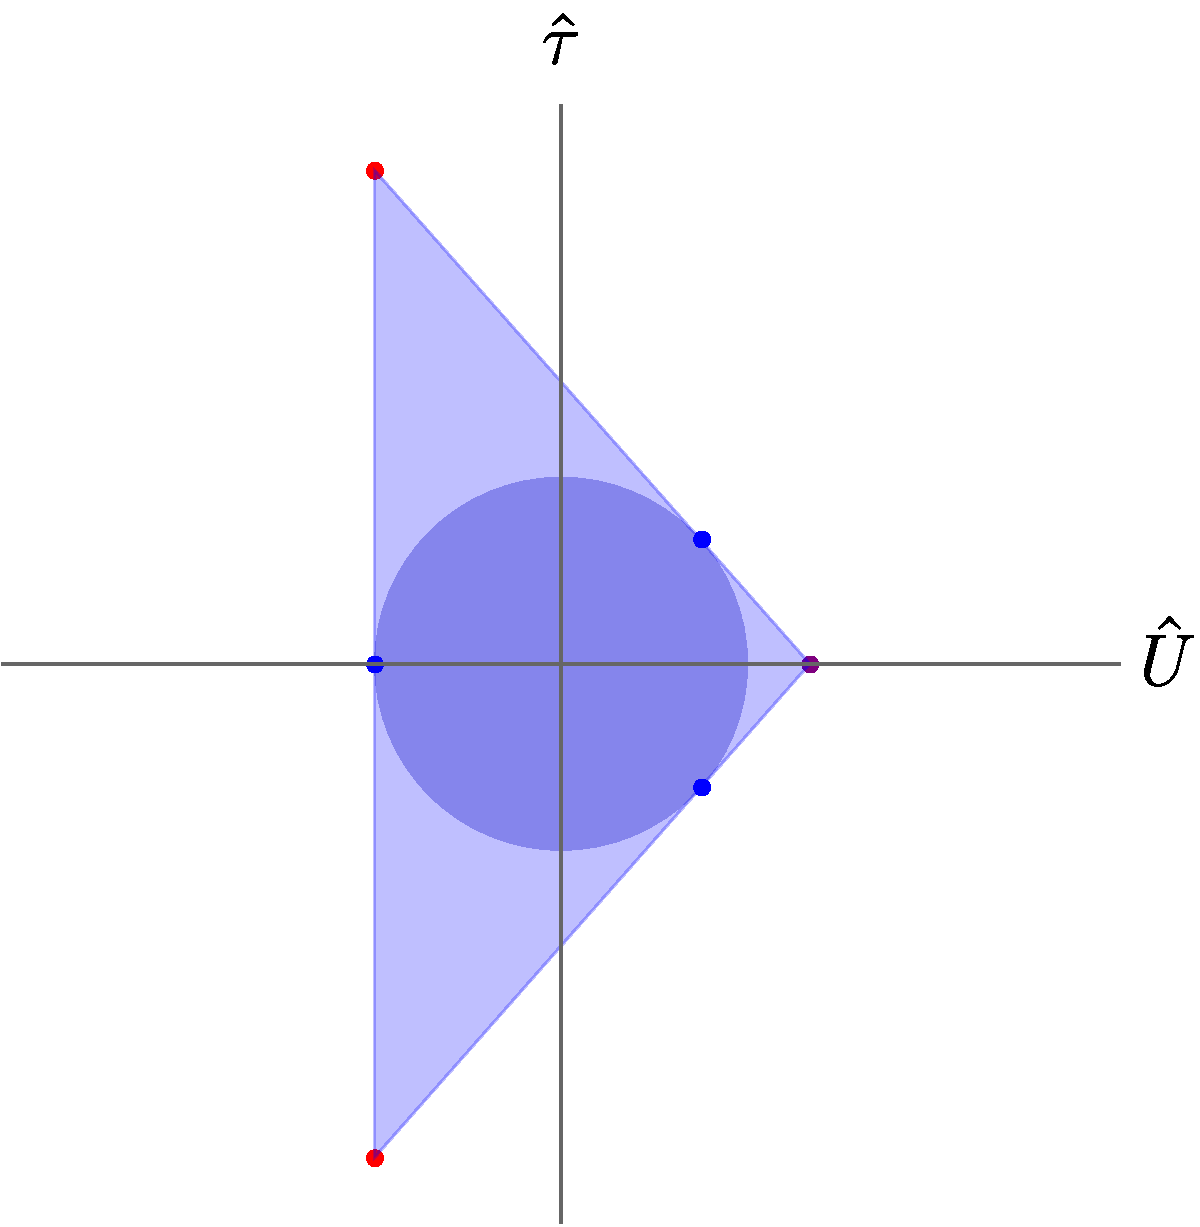
\includegraphics[width=0.45\textwidth]{CH-1-1.pdf}\label{sfig:9dCH}
			}
            \quad
			\subfigure[]{
				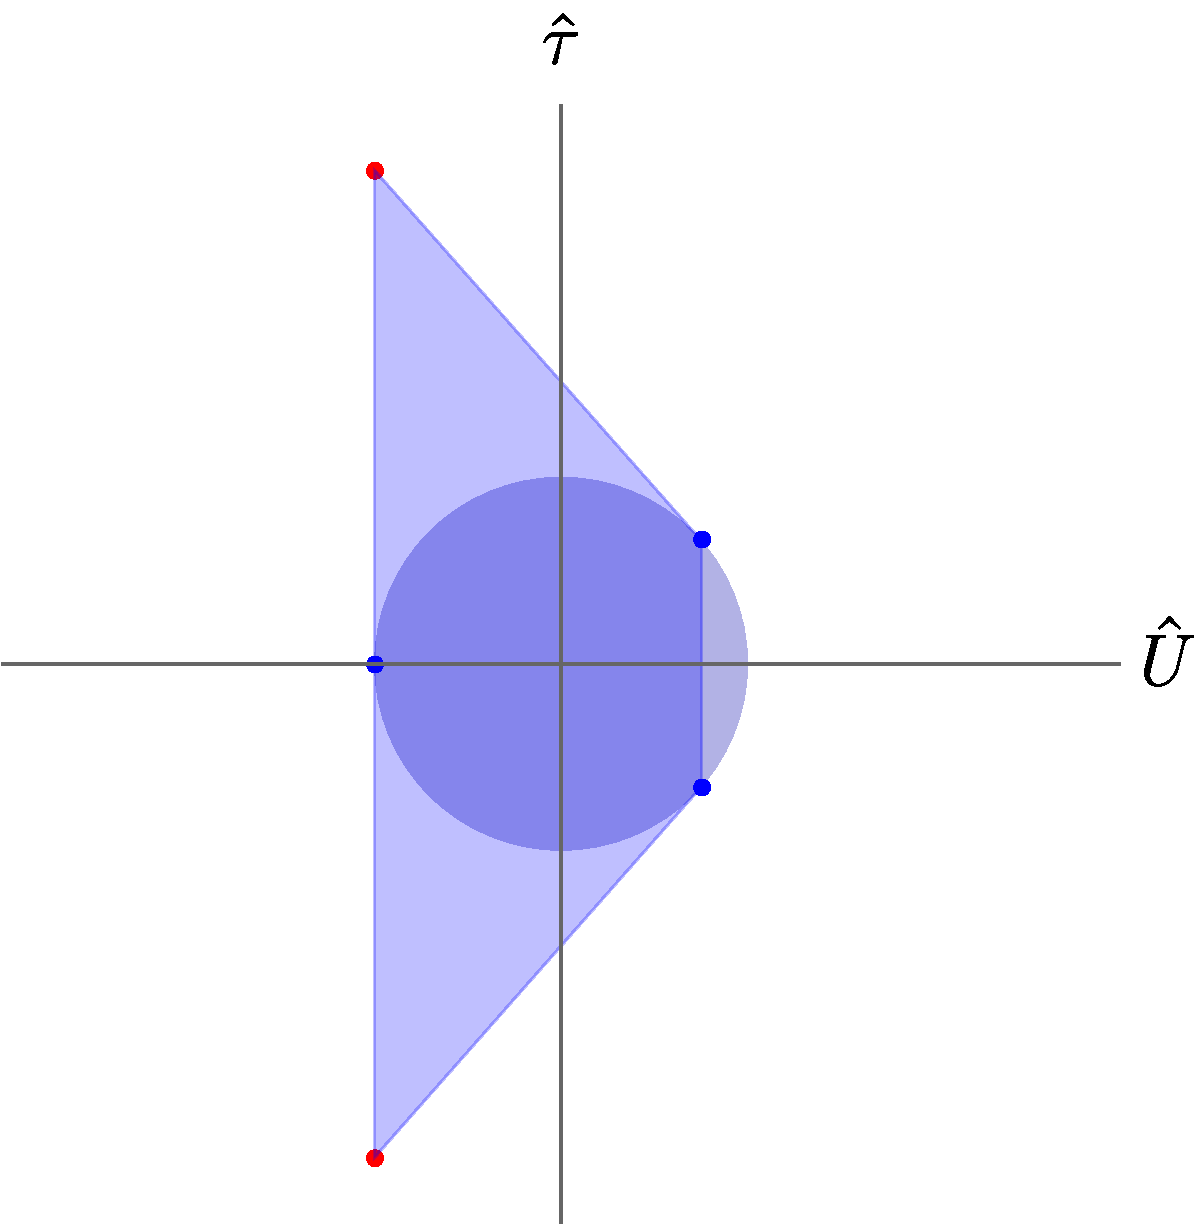
\includegraphics[width=0.45\textwidth]{CH-1-2.pdf}\label{sfig:9dCH-2}
			}
			\small \caption{\textbf{(a)} Convex hull condition for the species scale in M-theory on $\mathbf{T}^2$. \textbf{(b)} Convex hull condition for the species scale in M-theory on $\mathbf{T}^2$, if the effective double KK tower would not exist. The blue dots appearing in the edges of the convex hull are single KK towers, whereas the red and purple dots arising at the vertices represent stringy and double KK towers, respectively.}
			\label{fig:ch1}
		\end{center}
\end{figure} 
%%

Let us start with the vertices. Indeed, upon pointing towards any one of the red dots in Figure \ref{sfig:9dCH}, the species scale is dominated by a (critical) string tower. Therefore, the associated regime turns out to be an emergent string limit \cite{Lee:2019wij}. Similarly, for the direction determined by the purple dot, the species counting is saturated by the double KK tower, thus signalling towards full decompactification to 11d M-theory. In fact, this also holds upon exploring any intermediate direction between the blue dots in Figure \ref{sfig:9dCH}, since despite one KK tower being parametrically lighter than the other, the species scale is yet saturated by accounting for mixed states thereof (see discussion around eq. \eqref{eq:masseffectivetower}).

Finally, let us discuss the directions associated to the blue dots themselves. Notice that these vectors are always orthogonal to some edge of the convex hull. In fact, were not this the case, the condition \eqref{eq:bound9d} would be automatically violated since such single KK vectors precisely saturate the bound. This means, incidentally, that all three potential species scales lying at each edge of the convex hull fall at the same rate along the aforementioned limits, with their (finite) ratios not encoded in the convex hull and thus depending on the values of the moduli that are not sent to infinity. This fact has a nice physical interpretation: The species scale of the single Kaluza-Klein tower we are pointing to signals towards decompactification of one extra dimension, whereas the remaining pair of scales correspond to towers that are already present in the higher-dimensional theory. In fact, we observe that the edges precisely reproduce the (one-dimensional) convex hull of the decompactified theory. Indeed, the vertical line on the left-hand side of the diagram corresponds to the convex hull of 10d Type IIB string theory, with the F1 and D1-strings becoming light at weak and strong coupling, respectively. Similarly, the other two edges correspond to the convex hull of 10d Type IIA, with the fundamental string and the tower of D0-branes becoming light analogously at weak and strong coupling. 

In comparison with \cite{Etheredge:2022opl}, we also note that the roles of vectors saturating/protecting the convex hull condition are exchanged between strings and KK towers for the case of the species scale. This can be easily seen upon superimposing the diagrams for the $\zeta$- and $\mathcal{Z}$-vectors, as shown in Figure \ref{fig:ch2}. This moreover allows us to appreciate some hidden duality-like symmetry relating both convex hulls, which will be further investigated in Chapter \ref{ch:pattern} of this thesis.

%%%%%%%%%%%
\begin{figure}[htb]
\begin{center}
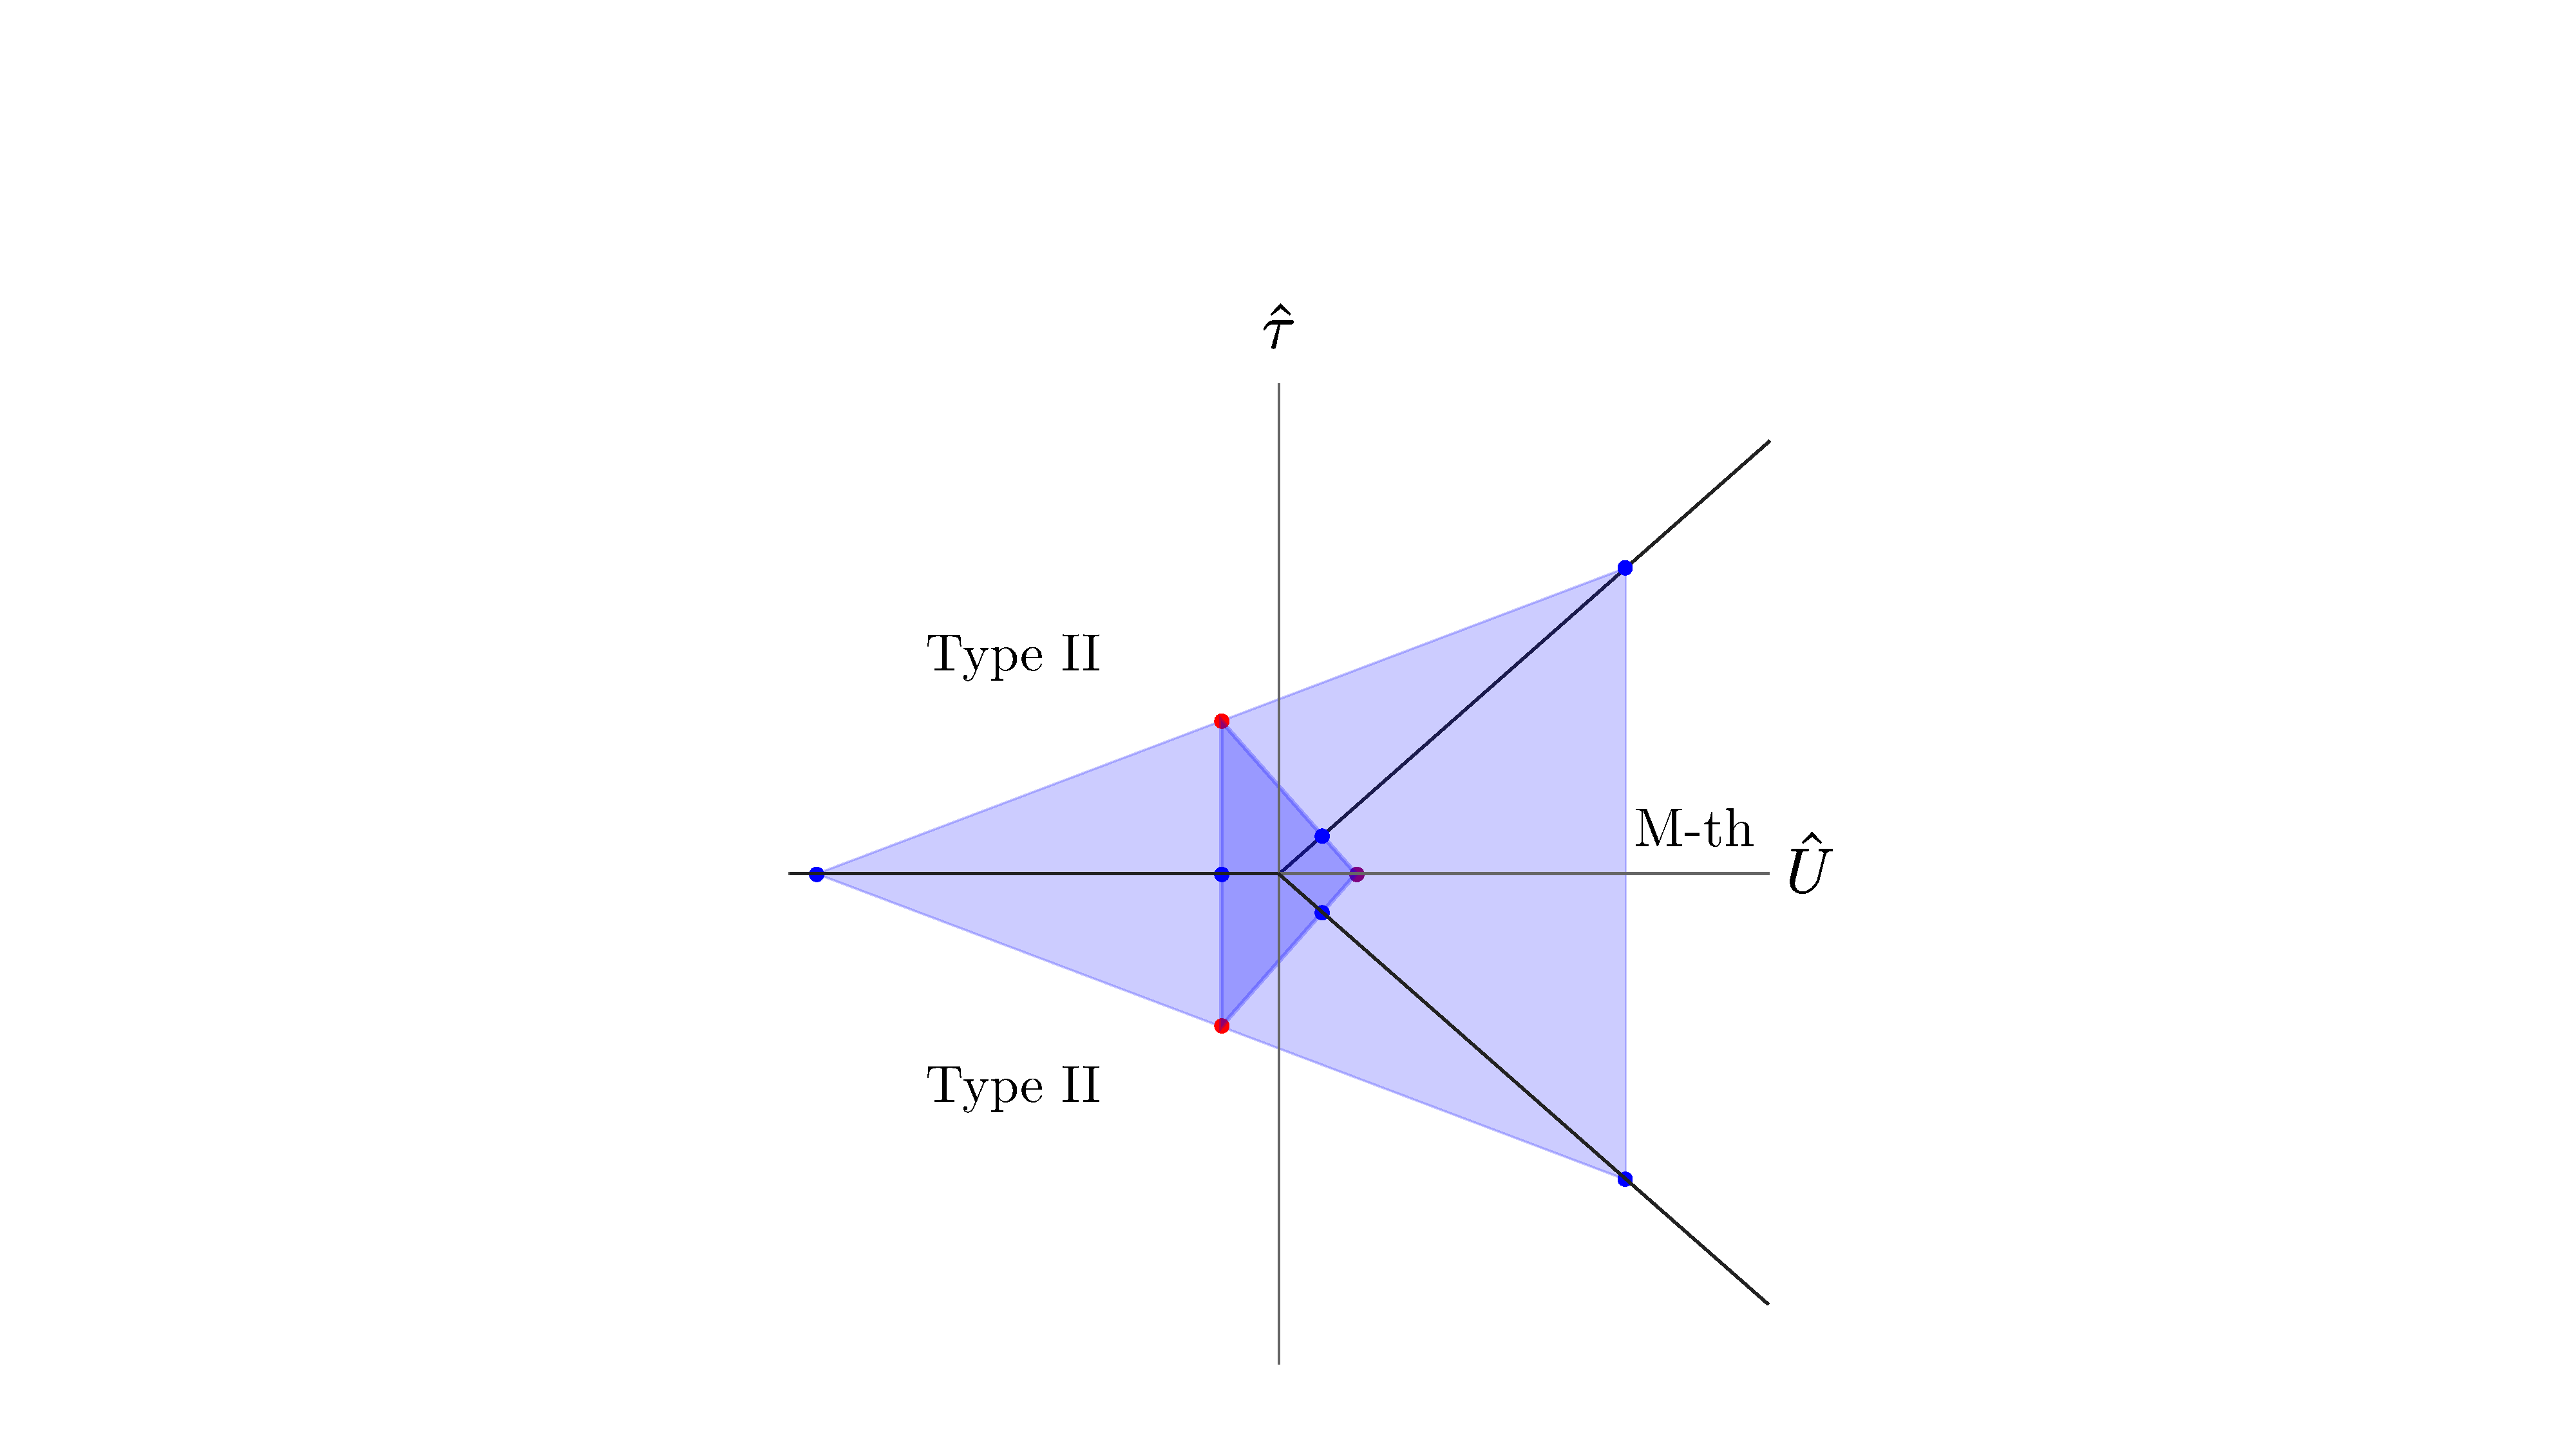
\includegraphics[width=0.45\textwidth]{CH-2.pdf}
\caption{\small Convex hulls superimposed for both the species scale and mass scales of the leading towers in M-theory on $\mathbf{T}^2$. The black lines separate the different duality frames within the 9d set-up, corresponding to Type II string theory and 11d M-theory. The self-dual line, at $\hat{\tau}=0$, is fixed under the $\mathbb{Z}_2$ remnant symmetry.} 
\label{fig:ch2}
\end{center}
\end{figure}
%%%%%%%%%%%

\subsubsection*{Revisiting the axion}
\label{sss:axions}

Before turning to our next string theory example, let us briefly reconsider the role of the axion $\tau_1$ in our previous discussion. This simple exercise proves to be instructive and teaches us a generic lesson on the significance of compact scalar fields in our analysis of the bound \eqref{eq:lowerboundspecies2}.

Notice from eq. \eqref{eq:9d} that the two scalar sectors of the theory are decoupled (at the two-derivative level) and only the modular one, which describes the complex structure of the internal $\mathbf{T}^2$, contains the axion. Such complex-valued field parametrizes the manifold $\mathsf{SL(2, \mathbb{Z})}\backslash \mathsf{SL(2, \mathbb{R})}/\mathsf{U(1)}$, with $\mathsf{SL(2, \mathbb{Z})}$ being the U-duality group of the 9d theory.

Restricting ourselves to the fundamental domain, $\mathscr{F}$, of the aforementioned moduli space (see Figure \ref{sfig:funddom} below) it is transparent that there is just one infinite distance singularity, namely $\tau \to \i \infty$. This corresponds to a weak coupling limit for the fundamental (F1) Type IIA string, whose tension reads
%
\begin{equation}\label{eq:IIAtension}
	T_{\text{F1}} = \frac{2\pi}{\ell_{9}^2} \frac{1}{\sqrt{\tau_2}}  \mathcal{V}_2^{\frac{3}{14}}\, ,
\end{equation}
%
leading to the species scale vector $\vec{\mathcal{Z}}_{\text{osc}} = \left(\left(\mathcal{Z}_{\rm osc}\right)_{U}, \left(\mathcal{Z}_{\rm osc}\right)_{\tau_2}, \left(\mathcal{Z}_{\rm osc}\right)_{\tau_1} \right)$ given by the components displayed in the first vector of equation \eqref{eq:speciesscalevectorsstringsT2}, together with an additional axionic component of the form
%
\begin{equation} \label{eq:chargetomassF1}
 \left(\mathcal{Z}_{\rm osc}\right)_{\tau_1} = -\frac{1}{2}\sqrt{G^{\tau_1 \tau_1}}\, \partial_{\tau_1} \log \left(T_{\text{F1}}\right) = 0 \, .%\\
\end{equation}
%
The fact that this extra component vanishes --- since the tension of the F1 does not depend on the axion --- implies that the decay rate parameter $\lambda_{\text{sp}}$ of the species scale along directions fulfilling $\tau \to \i \infty,\, U \to \infty$ is controlled just by the saxionic dependence of the species vector, regardless of the particular trajectory we follow so as to approach the weak coupling point. Furthermore, geodesics reaching infinity within $\mathscr{F}$ are given by vertical straight lines --- i.e. they satisfy $\dot \tau_1=\frac{d\tau_1}{d\sigma}=0$ with $\sigma \in \mathbb{R}$ some affine parameter --- such that we can effectively forget about the axionic direction $\tau_1$.

%%
\begin{figure}[htb]
		\begin{center}
			\subfigure[]{
				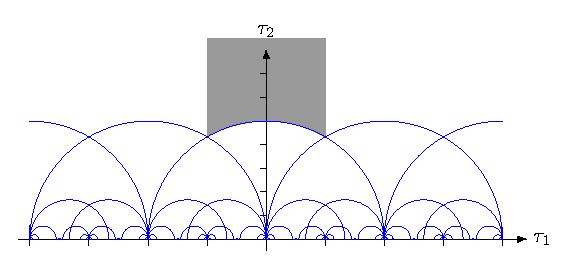
\includegraphics[width=0.5\textwidth]{FundamentalDomain.pdf}\label{sfig:funddom}
			}
            \quad
			\subfigure[]{
				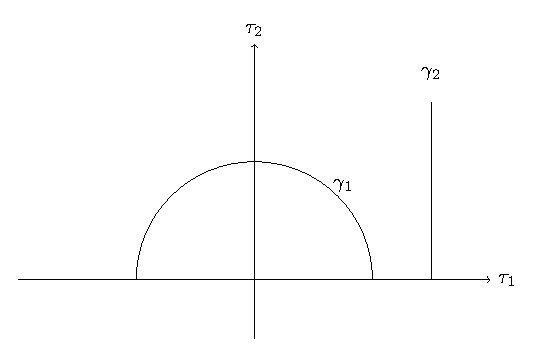
\includegraphics[width=0.425\textwidth]{Tikz_Hyperbolic_Lines.pdf}\label{sfig:geodesics}
			}
			\caption{\small \textbf{(a)} The upper half-plane $\mathbb{H}$ and the different $\mathsf{SL(2,\mathbb{Z})}$ domains one can consider, namely the `triangular' regions. The fundamental one $\mathscr{F}$ is shown shaded in grey. \textbf{(b)} Geodesics in the hyperbolic plane are given by vertical straight lines as well as half-circles intersecting the real axis at right angles.}
			
		\end{center}
\end{figure} 
%%

At this point, one could complain that the above conclusion might be an artifact of restricting ourselves to the fundamental domain, since the theory presents a whole plethora of $\frac{1}{2}$-BPS $(p,q)$-strings whose tension in Planck units is given by eq. \eqref{eq:pqstrings9d} above. Moreover, the latter actually provide for the dominant tower of light states required by the Distance Conjecture upon approaching different boundaries of the 9d moduli space, and are characterized by the following species vectors
%
\begin{equation} \label{eq:chargetomasspq}
\left(\mathcal{Z}_{p,q}\right)_{U} = -\frac{1}{2 \sqrt{14}} \, , \qquad	
 \left(\mathcal{Z}_{p,q}\right)_{\tau_2} = \frac{(p+q\tau_1)^2-q^2\tau_2^2}{2\sqrt{2} |p+q\tau|^2}\, , \qquad \left(\mathcal{Z}_{p,q}\right)_{\tau_1} =  -\frac{q \tau_2 (p+q\tau_1)}{\sqrt{2} |p+q\tau|^2}\, .
\end{equation}
%
In fact, it is easy to check --- taking also into account the $\tau_1$--\,direction --- that these vectors densely fill a circumference of radius $1/\sqrt{7}$, regardless of the particular point in moduli space we are sitting at \cite{Etheredge:2022opl}.\footnote{This point becomes subtle if one approaches an infinite distance boundary by taking e.g., $\tau_2 \to \infty$, since to actually fill the circumference one needs to consider $(p,q)$ bound states with increasingly bigger F1-string charge, namely $p \sim k \tau_2$ for $k\in \mathbb{Z}$, since otherwise their charge-to-mass vectors collapse to that of the F1 or D1-strings. Upon doing so, eq. \eqref{eq:chargetomasspq} leads to $\vec{\mathcal{Z}}_{p,q} = \frac{1}{\sqrt{8}} \left(\frac{1}{\sqrt{7}}, \cos 2\theta, -\sin 2\theta\right)$, with $\cos \theta =k/\sqrt{k^2+q^2}$.} This suggests that perhaps one might need to include the axionic component $\left(\mathcal{Z}_{p,q}\right)_{\tau_1}$ into our analysis, since it is non zero in general depending crucially on the value of $\braket{\tau_1}$. However, as we argue in what follows, the latter turns out to be irrelevant whenever we reach an asymptotic boundary of $\mathcal{M}_{\text{9d}}$. The reason being that for geodesic paths reaching an infinite distance singularity other than $\tau_2 \to \infty$, namely any point with $\tau_2=0$ and $\tau_1 \in \mathbb{Q}$ in Figure \ref{sfig:funddom}, one finds again both $\dot \tau_1 \to 0$ asymptotically as well as $\left(\mathcal{Z}_{p,q}\right)_{\tau_1} \to 0$ for the \emph{lightest} $(p,q)$-string. Indeed, the geodesic trajectories reaching such infinite distance points are given by half-circles orthogonal to the real axis with endpoint $(\tau_1, \tau_2)=(-p/q,0)$, see Figure \ref{sfig:geodesics}. Hence, upon substituting these values for $\tau_2$ and $\tau_1$ we obtain $\vec{\mathcal{Z}}_{p,q} \to \left(-\frac{1}{2 \sqrt{14}}, \frac{1}{2\sqrt{2}}, 0 \right)$, matching those from \eqref{eq:speciesscalevectorsstringsT2} and \eqref{eq:chargetomassF1}. As expected, this is merely a manifestation of the fact that an $\mathsf{SL(2, \mathbb{Z})}$ transformation relating F1 to any other $(p,q)$-string (i.e. their tensions) maps the vertical lines reaching $\i\infty$ to the circles intersecting the real axis at $\tau_1=-p/q$.

Therefore, the take-home message is that whenever we find some modular sector within the moduli space of our theory and we want to check whether the bound \eqref{eq:lowerboundspecies2} is satisfied \emph{asymptotically}, it is sufficient to restrict ourselves to the fundamental domain and focus just on the saxionic components of the species scale vectors. This follows since any other infinite distance path associated to a different $(p,q)$ tower can be effectively translated --- via some modular transformation --- to this simplified set-up. Notice that restricting to the fundamental domain means, in turn, that when plotting the convex hull in e.g., Figure \ref{sfig:9dCH} it is not necessary to consider directions exploring $\tau_2 \to 0$, since those are already accounted for once we sit in the appropriate duality frame.

\subsection{M-theory on $\mathbf{T}^3$}
\label{ss:MthyT3SSDC}

Let us now consider M-theory compactified on $\mathbf{T}^3$, yielding a 8d $\mathcal N=2$ supergravity effective field theory. The gravitational and scalar sectors are described by the following Einstein-frame action
%
\begin{align}\label{eq:8d}
	S_\text{M-th}^{\text{8d}}\, \supset\, &\frac{1}{2\kappa_8^2} \int \dd^{8}x\, \sqrt{-g}\,  \left( \mathcal{R} + \frac{1}{4} \text{tr} \left( \partial \tilde{g} \cdot \partial \tilde{g}^{-1} \right) -\frac{\partial \mathcal{T} \cdot \partial \bar{\mathcal{T}}}{2 \mathcal{T}_2^2} \right)\, ,
\end{align}
%
where $\tilde{g}_{m n}$ is related to the internal metric of the $\mathbf{T}^3$ and $\mathcal{T}=C_{123}^{(3)} + \text{i} \mathcal{V}_3$ is a complex field containing in particular the overall volume modulus (see Section \ref{ss:8dmaxsugra} for details). In this case, the U-duality group of the theory is enhanced to $\mathsf{SL(2, \mathbb{Z})} \times \mathsf{SL(3, \mathbb{Z})}$, with the above fields transforming in the adjoint representation of each of these factors. They moreover parametrize the group coset 
%
\begin{equation}\label{eq:8dmodspaceSSDC}
 \mathcal{M}_{\text{8d}}=\mathsf{SL(2, \mathbb{Z})}\backslash \mathsf{SL(2, \mathbb{R})}/\mathsf{U(1)} \times \mathsf{SL(3, \mathbb{Z})}\backslash \mathsf{SL(3, \mathbb{R})}/\mathsf{SO(3)}\, ,
\end{equation}
%

see discussion around eq. \eqref{eq:8dsl3}. The goal of this section is twofold: First we want to check that the convex hull condition 
%
\begin{equation} \label{eq:bound8d}
  \lambda_{\text{sp}} \geq \frac{1}{\sqrt{(d-1)(d-2)}} \stackrel{\text{8d}}{=} \frac{1}{\sqrt{42}}\, ,
\end{equation}
%
is indeed satisfied in the present set-up; and second we would like to understand how quantum gravity avoids the naive violation of the bound \eqref{eq:lowerboundspecies2} for the species scale in $D\leq9$, as discussed in our simple toy model from Section \ref{ss:compactificationstring} above. Of course, the mechanism by which this happens is precisely the appearance of new towers of light states along certain asymptotic directions, as will be verified later on. 

In principle, in order to check the condition \eqref{eq:bound8d} in full generality, one should take into account the dependence on the compact scalar fields (e.g., $ C_{123}^{(3)}= \text{Re}\, \mathcal{T}$) of the mass scale and $\zeta$-vectors associated to the infinite towers of states. However, for simplicity and in light of our analysis in nine dimensions, we will henceforth freeze all the axion fields in the theory, thus exploring geodesics in moduli space which move just along the non-compact directions. In any event, by making use of $\mathsf{SL(2, \mathbb{Z})} \times \mathsf{SL(3, \mathbb{Z})}$ duality, it is clear one can actually relate such trajectories to analogous ones exploring some other equivalent infinite distance singularity.

Therefore, following the logic of Section \ref{ss:compactificationstring}, let us rewrite the scalar lagrangian \eqref{eq:8d} as if it was obtained by circle-reduction from the 9d theory \eqref{eq:9d}, instead of compactifying M-theory directly on $\mathbf{T}^3$. Hence, we take the 9d metric in \eqref{eq:11dmetric} and propose the following ansatz
%
\begin{equation}\label{eq:9dmetric}
	ds^2_{9} = e^{-\sqrt{1/21}\,\rho} ds_8^2 + e^{\sqrt{12/7}\,\rho} \left(dy^3 \right)^2\, ,
\end{equation}
%
with the radion field $\rho$ being related to the extra radius by $R_3=e^{\sqrt{3/7}\,\rho}$. After dimensional reduction, one arrives at (c.f. eq. \eqref{eq:8dalternativeaction} for the full scalar action) 
%
\begin{equation}\label{eq:8dcanonical}
	S^{\text{8d}}_{\text{M}} \supset \frac{1}{2\kappa_8^2} \int \dd^{8}x\, \sqrt{-g}\,  \left( \mathcal{R} - \left( \partial \hat U \right)^2 - \left(\partial \hat \tau\right)^2 - \left( \partial \hat \rho \right)^2 \right) + \left( \text{axions} \right)\, ,
\end{equation}
%
where we have introduced the canonically normalized radion $\hat \rho=\frac{\rho}{\kappa_8 \sqrt{2}}$ as well as those defined in \eqref{eq:canonicalnormalization}. Note that the compactification process just described can be equivalently seen as a $\mathbf{T}^2$-fibration over $\mathbf{S}^1$.

With this, we can now start computing the mass scales of the infinite tower of states, their charge-to-mass vectors $\vec{\zeta}$, as well as their (combined) species scales, similarly to what we did in the 9d setting. The relevant towers are shown in Table \ref{tab:BPSstates}. 
%%%%%%%%%%%%%%%%%%%%%%%%%%%%%%%
\begin{table}[tb]\begin{center}
\renewcommand{\arraystretch}{2.00}
\begin{tabular}{|c|c|c|c|}
\hline BPS states & Microscopic interpretation & Tension & Multiplicity \\
\hline \hline 
strings &  M2 on $\mathbf{S}^1_i$  &    $T = \frac{2 \pi}{\ell_{11}^3} (2\pi\, \mathsf{R}_i)$  &   $3$ \\
particles (non-pert.) & M2 on $\mathbf{S}^1_i \times \mathbf{S}^1_j$  &    $m_{\text{M2}} = \frac{2 \pi}{\ell_{11}^3} (4\pi^2\, \mathsf{R}_i\, \mathsf{R}_j)$  &   $3$ \\
particles (pert.) &  KK from $\mathbf{S}^1_i$  &    $m_{\text{KK}}= \frac{1}{\mathsf{R}_i}$  &   $3$\\
\hline
\end{tabular}
\caption{Relevant towers of $\frac{1}{2}$-BPS states in M-theory on $\mathbf{T}^3$. Their mass/tension is computed in terms of the dimensionful radii $\mathsf{R}_i$ and the 11d Planck length $\ell_{11}$.}
  \label{tab:BPSstates}
  \end{center}\end{table} 
%%%%%%%%%%%%%%%%%%%%%%%%%%%%%%%

\begin{comment}
%%%%%%%%%%%%%%%%%%%%%%%%%%%%%%%
	\begin{table}[h!!]\begin{center}
			\renewcommand{\arraystretch}{1.00}
			\begin{tabular}{|c|c|c|c|}
				\hline
				BPS states &  Microscopic int.  &  Tension/Mass  & Degeneracy  \\
				\hline 
				strings&  M2 on $\mathbf{S}^1_i$  &    $T \propto (2\pi R_i)$  &   $3$ \\
				\hline
				non-perturbative particles & M2 on $\mathbf{S}^1_i \times \mathbf{S}^1_j$  &    $m_{\text{M2}} \propto (2\pi R_i)(2\pi R_j)$  &   $3$ \\
				\hline
				perturbative particles &  KK from $\mathbf{S}^1_i$  &    $m_{\text{KK}}= 1/ R_i$  &   $3$\\
				% \hline
				% instantons & M2 on $T^3$  &  $S_{\text{M2}} \propto R_1 R_2 R_3$  
    %             &   1  \\
				\hline
			\end{tabular}
			\caption{Relevant towers of $\frac{1}{2}$-BPS states together with their mass scales (in Planck units) in M-theory on $\mathbf{T}^3$.}
			\label{tab:BPSstates}
		\end{center}
	\end{table}
 %%%%%%%%%%%%%%%%%%%%%%%%%%%%%%%%%
 \end{comment}
 
%Notice that apart from the states discussed in that section, we get an additional\footnote{There are other BPS extended objects in the theory, such as M5-branes and descendants obtained from wrapping it along different cycles of the $T^2$ manifold. We refuse to discuss their multiplicity and kinematics since they play no role in our present discussion.} M2-brane with tension
%
%\begin{equation}\label{eq:9dM2}
%	T_{\text{M2}} \sim \frac{2\pi}{\ell_9^3} e^{-3U/7} \sim \frac{2\pi}{\ell_9^3} e^{-2\hat U/\sqrt{14}}\, ,
%\end{equation}
%
%where $\ell_9$ denotes the nine-dimensional Planck length.

Let us first study the case of solitonic critical strings. It is easy to see that apart from the set of $(p,q)$-strings which were already present in nine dimensions, we get an additional one by wrapping the M2-brane along the extra $\mathbf{S}^1$, whose tension is given by
%
\begin{equation}\label{eq:8dstring}
	T_{\text{str}''} =  \frac{2\pi}{\ell_8^2} e^{-2\hat U/\sqrt{14}}\, e^{2\sqrt{2}/\sqrt{21}\, \hat \rho} \quad \Longrightarrow \quad \frac{m_{\text{osc}''}}{M_{\text{Pl};\, 8}}  \sim e^{-\frac{1}{\sqrt{14}}\hat U}\, e^{\sqrt{\frac{2}{21}}\, \hat \rho}\, .
\end{equation}
%
Therefore, upon taking this extra M2-string into account, we arrive at the following species vectors associated to towers of oscillator modes
%
\begin{equation} \label{eq:stringvectors}
\begin{split} 
	\vec{\mathcal{Z}}_{\text{osc}} &= \left( \frac{1}{2\sqrt{2}} , \frac{1}{\sqrt{42}}, -\frac{1}{2 \sqrt{14}} \right)\, , \qquad \vec{\mathcal{Z}}_{\text{osc}'} = \left( -\frac{1}{2\sqrt{2}} , \frac{1}{\sqrt{42}}, -\frac{1}{2 \sqrt{14}} \right) \, ,\\
	\vec{\mathcal{Z}}_{\text{osc}''} &= \left( 0 , -\sqrt{\frac{2}{21}}, \frac{1}{\sqrt{14}} \right) \, ,
\end{split}
\end{equation}
%
where we have adopted the notation $\vec{\mathcal{Z}} = \left(\mathcal{Z}_{\hat \tau}, \mathcal{Z}_{\hat \rho}, \mathcal{Z}_{\hat U} \right)$. To obtain the first two we made use of eq. \eqref{string-species} together with the second relation in \eqref{eq:zvectorafterdimreduction}. Notice that they satisfy $|\vec{\mathcal{Z}}_{\text{osc}}|^2=1/(d-2)=1/6$, as expected. Physically, these strings can be interpreted as a fundamental Type IIA string and S-duals thereof by choosing one reference 1-cycle as the M-theory circle.

For the Kaluza-Klein towers, we proceed analogously to the string case above, namely we borrow the results from the 9d set-up and then compute the additional KK scale associated to the extra circle. One then finds
%
\begin{equation} \label{eq:KKvectors}
\begin{split} 
	\vec{\mathcal{Z}}_{\text{KK},\, 1} &= \left( \frac{1}{7\sqrt{2}} , \frac{1}{7 \sqrt{42}}, \frac{3}{7 \sqrt{14}} \right) \, , \qquad \vec{\mathcal{Z}}_{\text{KK},\, 1'} = \left( -\frac{1}{7\sqrt{2}} , \frac{1}{7 \sqrt{42}}, \frac{3}{7 \sqrt{14}} \right) \, ,\\
	\vec{\mathcal{Z}}_{\text{KK},\, 1''} &= \left( 0 , \frac{1}{\sqrt{42}}, 0 \right) \, .
\end{split}
\end{equation}
%
Note that all these vectors verify $|\vec{\mathcal{Z}}_{\text{KK}}|^2=1/(d-1)(d-2)=1/42$, thus saturating the bound \eqref{eq:bound8d}. In string theory language, they become two distinct KK towers and (bound states of) D0-branes upon choosing --- without loss of generality --- some $\mathbf{S}^1$ as the M-theory circle. Moreover, the first two vectors, which were already present in nine dimensions, have some $\lambda_{\text{sp}}$--\,parameter whose functional form is preserved upon dimensional reduction, in agreement with our claims from Section \ref{s:consistencydimreduc}.

Lastly, the other relevant set of $\frac{1}{2}$-BPS particles arises from M2-branes wrapping any 2-cycle of the internal manifold, as shown in Table \ref{tab:BPSstates}. These can be either seen as winding modes associated to each one of the three critical strings displayed in \eqref{eq:stringvectors}, or alternatively, as the 8d analogues of the F-theory tower discussed around eq. \eqref{eq:Ftheorytower}. In any event, it is clear that they are nothing but KK towers associated to decompactification limits in a dual Type IIB frame. Their species vectors can be easily computed to be
%
\begin{equation} \label{eq:M2vectors}
\begin{split} 
	\vec{\mathcal{Z}}_{\text{M},\, 1} &= \left( \frac{1}{7\sqrt{2}}, -\frac{5}{7 \sqrt{42}}, -\frac{1}{7 \sqrt{14}} \right) \, , \qquad \vec{\mathcal{Z}}_{\text{M},\, 1'} = \left( -\frac{1}{7\sqrt{2}}, -\frac{5}{7 \sqrt{42}}, -\frac{1}{7 \sqrt{14}} \right) \, ,\\
	\vec{\mathcal{Z}}_{\text{M},\, 1''} &= \left( 0, \frac{1}{7 \sqrt{42}}, -\frac{\sqrt{8}}{7 \sqrt{7}} \right)\, .
\end{split}
\end{equation}
%
which verify $|\vec{\mathcal{Z}}_{\text{M}}|^2=1/(d-1)(d-2)=1/42$ as well. 

We are not done yet, though. As we learned from the general analysis of Section \ref{s:consistencydimreduc} and the 9d example above, one needs to take into account effective combinations of towers of states, whose associated species scale can be lower than naively expected. For the case at hand, the ones that will be relevant are those formed by bound states involving only Kaluza-Klein replica, those comprised by M2-particles alone and a mixture of these two sectors. The KK bound states lead to the following set of vectors
%
\begin{equation} \label{eq:KKvectorscombined}
\begin{split} 
	\vec{\mathcal{Z}}_{\text{KK},\,2} &=  \left( 0, \frac{1}{4 \sqrt{42}}, \frac{3}{4 \sqrt{14}} \right) \, , \qquad \qquad \, \vec{\mathcal{Z}}_{\text{KK},\,2'} =  \left( \frac{1}{8 \sqrt{2}}, \frac{1}{ \sqrt{42}}, \frac{3}{8 \sqrt{14}} \right) \, ,\\
	\vec{\mathcal{Z}}_{\text{KK},\,2''} &=  \left( -\frac{1}{8 \sqrt{2}}, \frac{1}{ \sqrt{42}}, \frac{3}{8 \sqrt{14}} \right) \, , \qquad \vec{\mathcal{Z}}_{\text{KK},\,3} =  \left( 0, \frac{1}{ \sqrt{42}}, \frac{2}{3 \sqrt{14}} \right) \, .
\end{split}
\end{equation}
%
whilst for the M2-particles one finds instead
%
\begin{equation} \label{eq:M2vectorscombined}
\begin{split} 
	\vec{\mathcal{Z}}_{\text{M},\, 2} &=  \left( 0, -\frac{5}{4 \sqrt{42}}, -\frac{1}{4 \sqrt{14}} \right) \, , \qquad \qquad \ \ \vec{\mathcal{Z}}_{\text{M},\, 2'} =  \left( \frac{1}{8 \sqrt{2}}, -\frac{1}{ 2 \sqrt{42}}, -\frac{5}{8 \sqrt{14}} \right) \, ,\\
	\vec{\mathcal{Z}}_{\text{M},\, 2''} &=  \left( -\frac{1}{8 \sqrt{2}}, -\frac{1}{ 2 \sqrt{42}}, -\frac{5}{8 \sqrt{14}} \right) \, , \qquad \vec{\mathcal{Z}}_{\text{M},\, 3} =  \left( 0, -\frac{1}{ \sqrt{42}}, -\frac{2}{3 \sqrt{14}} \right) \, ,
\end{split}
\end{equation}
%
Finally, one can construct effective BPS towers of M2-particles with non-trivial KK momentum along the 1-cycle they do not wrap. These will be denoted as
%
\begin{equation} \label{eq:KK&M2vectorscombined}
\begin{split} 
	\vec{\mathcal{Z}}_{\text{KK-M},\, 2} &=  \left( 0, \frac{1}{\sqrt{42}}, -\frac{1}{2 \sqrt{14}} \right) \, , \qquad \vec{\mathcal{Z}}_{\text{KK-M},\, 2'} =  \left( -\frac{1}{4 \sqrt{2}}, -\frac{1}{2 \sqrt{42}}, \frac{1}{4 \sqrt{14}} \right) \, ,\\
	\vec{\mathcal{Z}}_{\text{KK-M},\, 2''} &=  \left( \frac{1}{4 \sqrt{2}}, -\frac{1}{2 \sqrt{42}}, \frac{1}{4 \sqrt{14}} \right) \, .
\end{split}
\end{equation}
%
The physical interpretation of the species scales associated to the vectors \eqref{eq:KKvectorscombined}-\eqref{eq:KK&M2vectorscombined} is straightforward: The first three of each set can be seen to be effective towers with density parameter $p=2$, such that they satisfy $|\vec{\mathcal{Z}}_{\rm sp}|^2=1/24$ and moreover implement some double decompactification to ten dimensions (possibly in a dual frame). On the other hand, the last vector of both eqs. \eqref{eq:KKvectorscombined} and \eqref{eq:M2vectorscombined} take us back to 11d M-theory, and as such verify $|\vec{\mathcal{Z}}_{\text{KK},\,3}|^2=|\vec{\mathcal{Z}}_{\text{M},\,3}|^2=1/18$. %The triplet \eqref{eq:KK&M2vectorscombined} also implement some double decompactification to 10d.

\subsubsection*{Plotting the convex hull}

Once we have all the $\mathcal{Z}$-vectors associated to the individual species scales, we can plot them in a 3d graph to check whether the CHC is satisfied or not. This is shown in Figure \ref{fig:ch8dgeneric} from two different perspectives, where one can see very explicitly that the convex hull for the present 8d example contains the ball of radius $\frac{1}{\sqrt{42}}$, thus fulfilling the bound \eqref{eq:lowerboundspecies2}. 

%%%%%%%%%%%%%%%%%%
\begin{figure}[htb]
		\begin{center}
			\subfigure[]{
				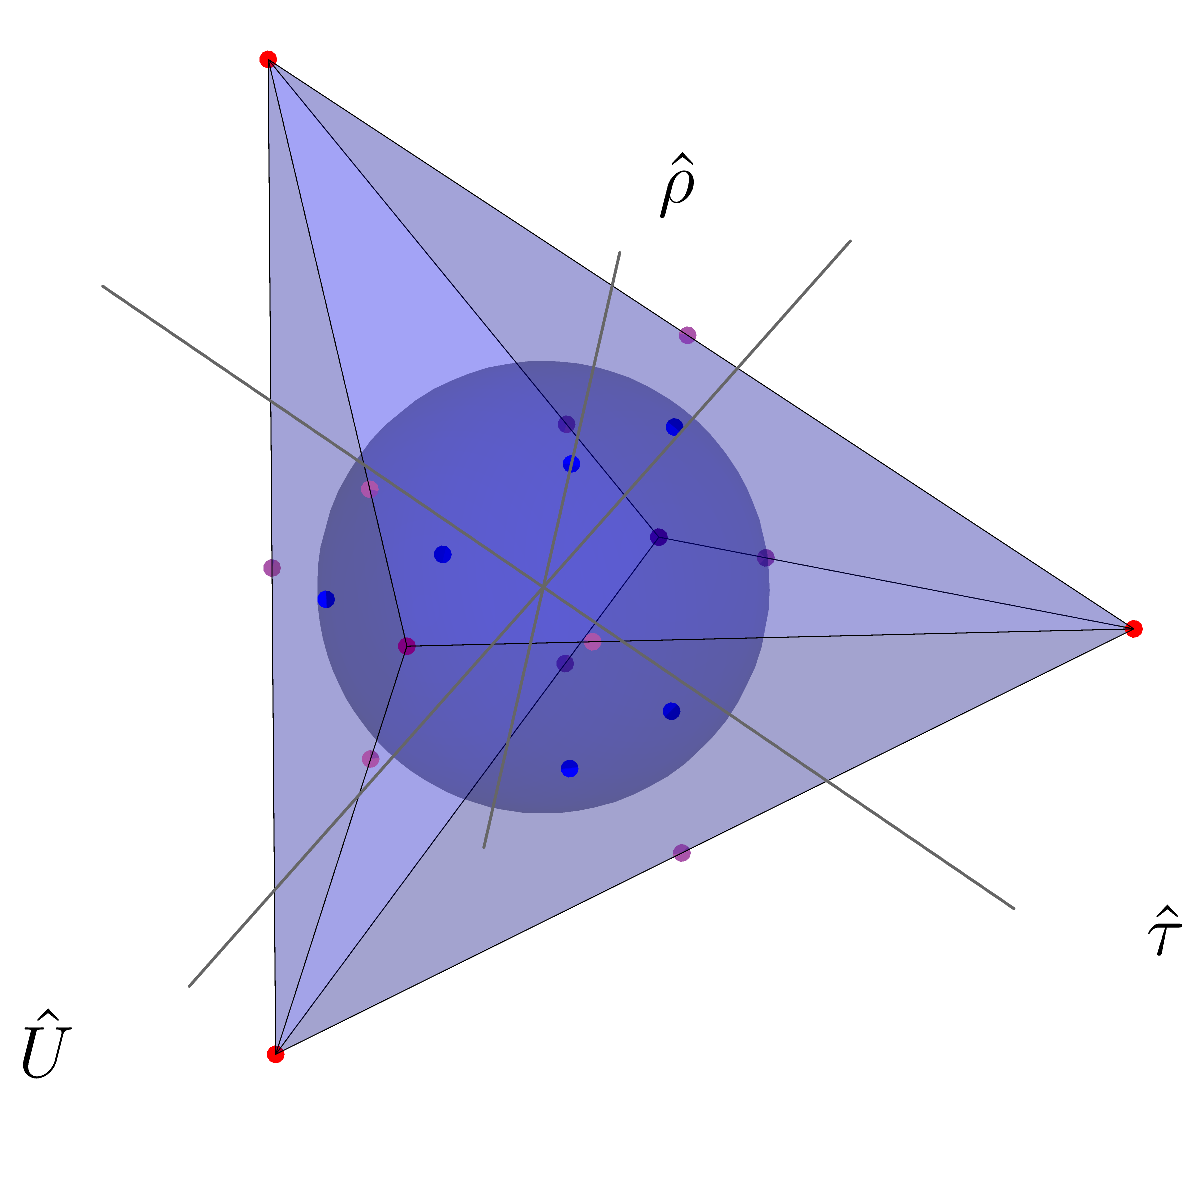
\includegraphics[width=0.45\textwidth]{CH-T3-1.pdf}\label{sfig:slice3dCH}
			}
			\subfigure[]{
				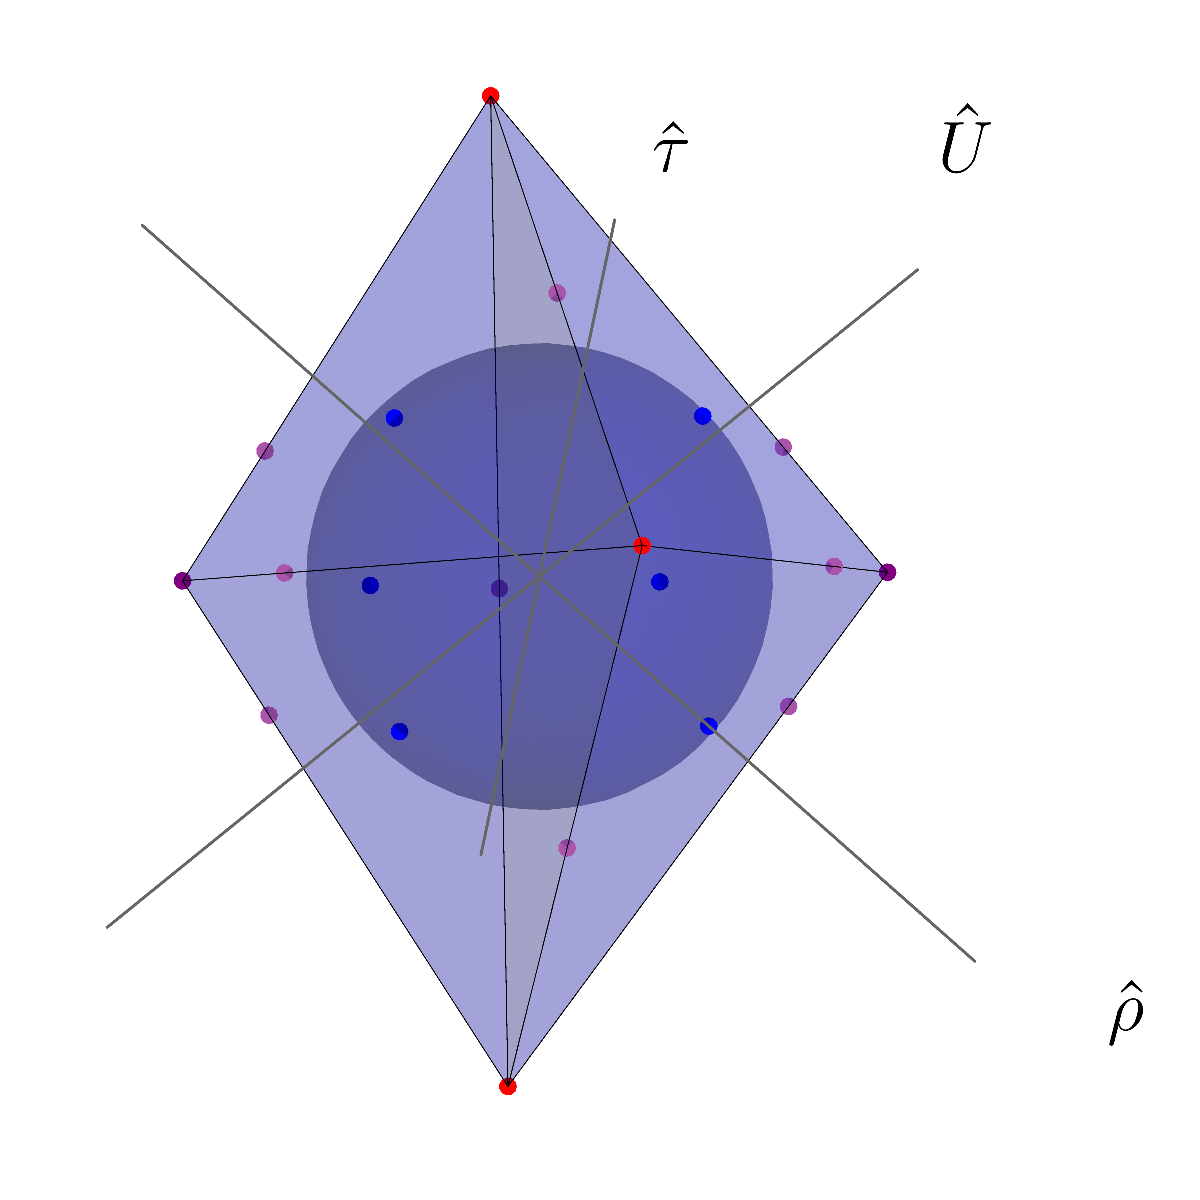
\includegraphics[width=0.45\textwidth]{CH-T3-2.pdf}\label{sfig:2ndslice3dCH}
			}
			\caption{\small Convex hull for the species scale in M-theory on $\mathbf{T}^3$ with the axions set to a constant value, as seen from two different angles. The blue dots in the faces of the resulting polyhedron correspond to single KK towers ($p=1$), the light purple dots in the edges indicate double KK towers ($p=2$) and the dark purple and red dots in the vertices correspond to triple KK towers ($p=3$) and string towers, respectively.}
			\label{fig:ch8dgeneric}
		\end{center}
\end{figure} 
%%%%%%%%%%%%%%%%%%

Interestingly, and similarly to what happened in the 9d setting discussed in Section \ref{ss:MthyT2SSDC}, the convex hull diagram for the species vectors features various nice properties capturing both the symmetries of the quantum theory as well as the relevant physics associated to the infinite distance boundaries in $\mathcal{M}_{\text{8d}}$. Indeed, from Figure \ref{sfig:2ndslice3dCH} (see also Figure \ref{fig:ch8dSL3} below) one can easily spot a surviving $\mathsf{S}_3 \times \mathsf{S}_2$ symmetry, where $\mathsf{S}_n$ denotes the permutation group of $n$ elements. Such discrete group can be thought of as a remnant of the U-duality group existing in the full eight-dimensional theory (see footnote \ref{fnote.Weyl} for more on this). In fact, this implies that the convex hull for the species scale is completely encoded within some \emph{fundamental domain} $\mathscr{F}_{8}$, which is replicated by acting on it with different elements of the discrete symmetry group. This latter observation will be crucial later on in Section \ref{ss:MthyTk} so as to extend the present analysis to set-ups with maximal supersymmetry in $d<8$.

%%%%%%%%%%%%
\begin{figure}[htb]
\begin{center}
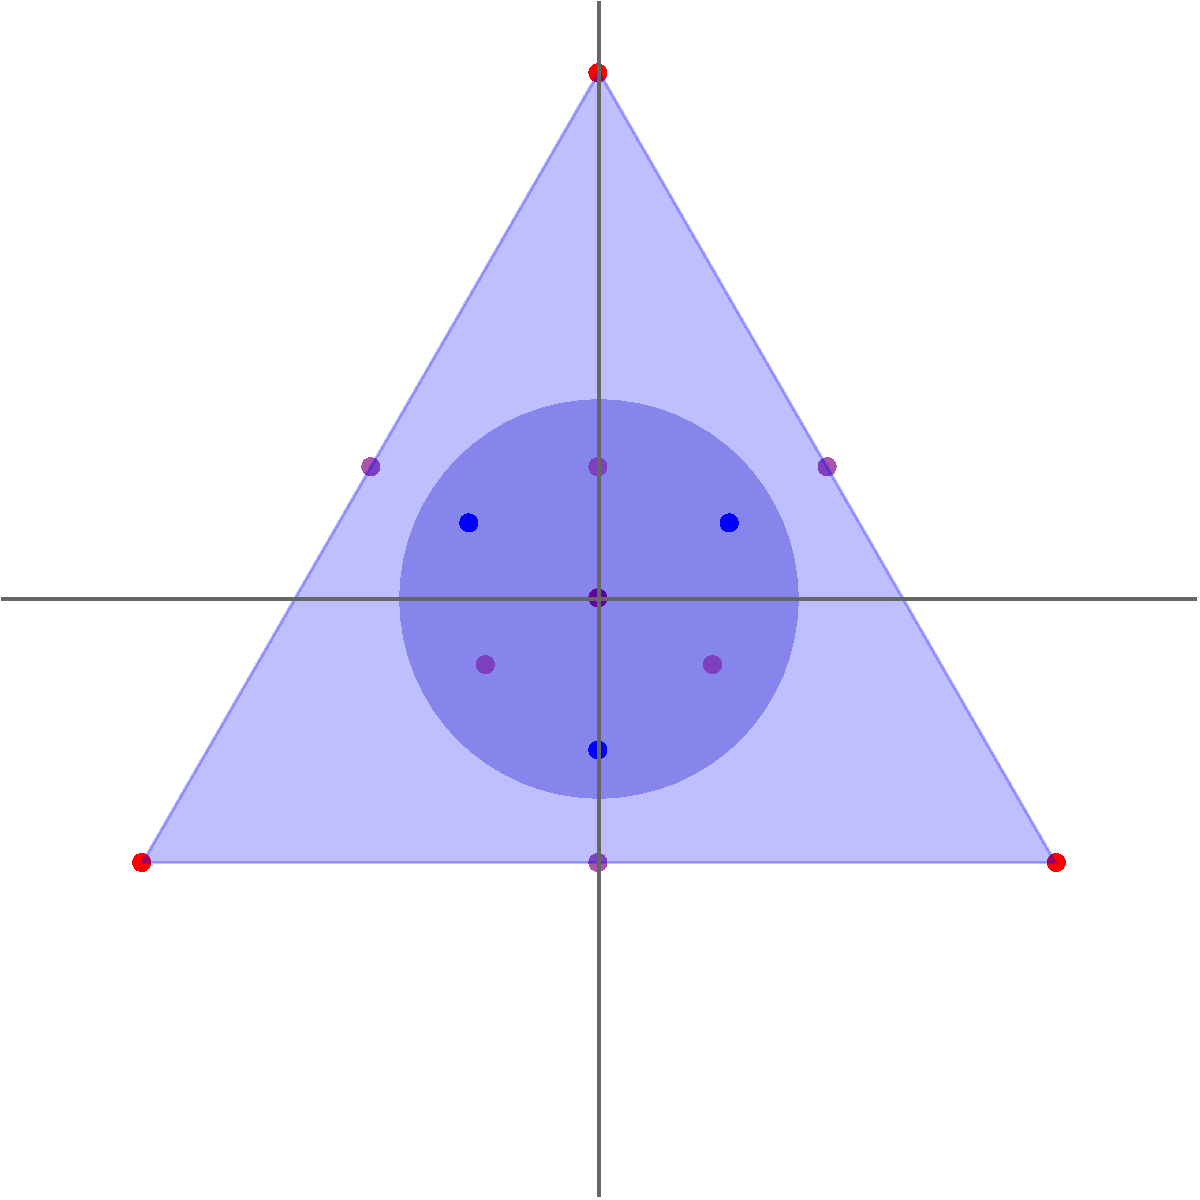
\includegraphics[scale=.4]{CH-T3-projected-2.pdf}
\caption{\small Two-dimensional projection of the convex hull for the species scale in M-theory on $\mathbf{T}^3$. The slice is chosen with respect to the normal vector $\hat T = \frac{\vec{\mathcal{Z}}_{\text{KK},\, 3}}{|\vec{\mathcal{Z}}_{\text{KK},\, 3}|}$, making thus manifest the discrete symmetry remnant of the $\mathsf{SL(3, \mathbb{Z})}$ duality (sub-)group.} 
 \label{fig:ch8dSL3}
 \end{center}
 \end{figure}
 %%%%%%%%%%%%

Regarding the structure exhibited by the diagram, let us first notice that the convex hull is fully generated again by the species vectors associated to either emergent string limits (the red dots in Figure \ref{fig:ch8dgeneric}) or full decompactification to 11d M-theory (the purple dots). On the other hand, the vectors marked by blue dots, corresponding to $p=1$ towers, saturate the constraint \eqref{eq:bound8d} and appear precisely at the faces of the convex polyhedron, being moreover perpendicular to the latter. In fact, these faces turn out to be nothing but the convex hull diagram of the `parent' 9d theory (see Figure \ref{sfig:9dCH-2}), which in turn include at its edges the convex hull for the different limiting 10d theories. Therefore, we find an inductive sequence of the form
%
\beq
    {\rm Hull}\left(\{\vec{\mathcal{Z}}_I\}\right)\big\rvert_{\rm 8d} \supset {\rm Hull}\left(\{\vec{\mathcal{Z}}_I\}\right)\big\rvert_{\rm 9d} \supset {\rm Hull}\left(\{\vec{\mathcal{Z}}_I\}\right)\big\rvert_{\rm 10d} \supset {\rm Hull}\left(\{\vec{\mathcal{Z}}_I\}\right)\big\rvert_{\rm 11d}\, ,
\eeq
%
informing us about all possible infinite distance limits that can be explored either directly from the lower dimensional perspective, or rather by passing first through some intermediate higher-dimensional frame.  

\subsubsection*{Comparison with the toy model}

Finally, in order to appreciate the crucial role played by the effective towers of states so as to ensure that the convex hull condition to be verified, let us study one concrete 2d slice of Figure \ref{fig:ch8dgeneric}, namely the one spanned by the $\{\hat \rho, \hat \tau \}$ directions. Hence, upon projecting the $\mathcal{Z}$-vectors down to a plane characterized by its normal $\hat T = \partial_{\hat{U}}$ as follows
%
\begin{equation}\label{eq:2dprojection}
	\vec{\mathcal{Z}}_{\hat T} = \vec{\mathcal{Z}} - \left( \hat T \cdot \vec{\mathcal{Z}}\right) \hat T\, ,
\end{equation}
%
one obtains precisely what is shown in Figure \ref{fig:ch-comparison-toymodel} below. The reason for choosing this particular slice is because it can be easily connected to the situation discussed previously in Section \ref{ss:compactificationstring}. There we showed that, upon compactifying a $D$-dimensional theory containing two S-dual strings on a circle, the CHC seemed to be naively violated whenever $D\leq9$. Indeed, the lower-dimensional vectors associated to the pair of strings together with their winding modes --- and effective combinations thereof, which are crucial to satisfy \eqref{eq:lowerboundspecies2} if $D=10$, were actually not sufficient to preserve the latter when starting from the non-critical dimension (c.f. Figure \ref{sfig:9dto8d}). On the other hand, if we consider M-theory on $\mathbf{T}^3$ instead, which of course provides for an eight-dimensional EFT coming from quantum gravity, there is indeed no violation of the CHC. In fact, the projected 2d slice of the hull depicted in Figure \ref{fig:ch-comparison-toymodel} turns out to have a similar structure to the one exhibited by the toy model, which is also shown for comparison. Indeed, in both cases there are two strings that correspond to the red dots appearing in the upper half of the image, which are connected by a line that is tangent to the critical ball of radius $\frac{1}{\sqrt{42}}$. The saturation happens precisely along the asymptotic direction where the KK tower associated to the extra $\mathbf{S}^1$ becomes relevant. In the opposite regime, namely along the negative $\hat \rho$ axis, where the (effective) tower of winding modes do not give rise to a convex hull containing the critical ball, a genuine 8d critical string appears in M-theory (i.e. the one in eq. \eqref{eq:8dstring}). It is precisely this new tower of oscillator modes, which was absent in the toy model, the one ensuring that the bound is preserved along every direction in the resulting 2d graph.

%From the previous discussion one can draw a couple of nice lessons. First, as expected based on general considerations in Section \ref{ss:compactificationstring}, upon compactifying to lower dimensions one starts to need from genuine QG ingredients in order to satisfy the CHC, namely new infinite towers of states. In a sense, from a bottom-up perspective, one could say that the naive imposition of the convex hull condition to certain directions in this 8d set-up \emph{postdicts} the existence of new infinite distance limits, which turn out to have a nice UV embedding from the 11d perspective.

%%%%%%%%%%%%
\begin{figure}[htb]
\begin{center}
	\subfigure[M-theory on $\mathbf{T}^3$]{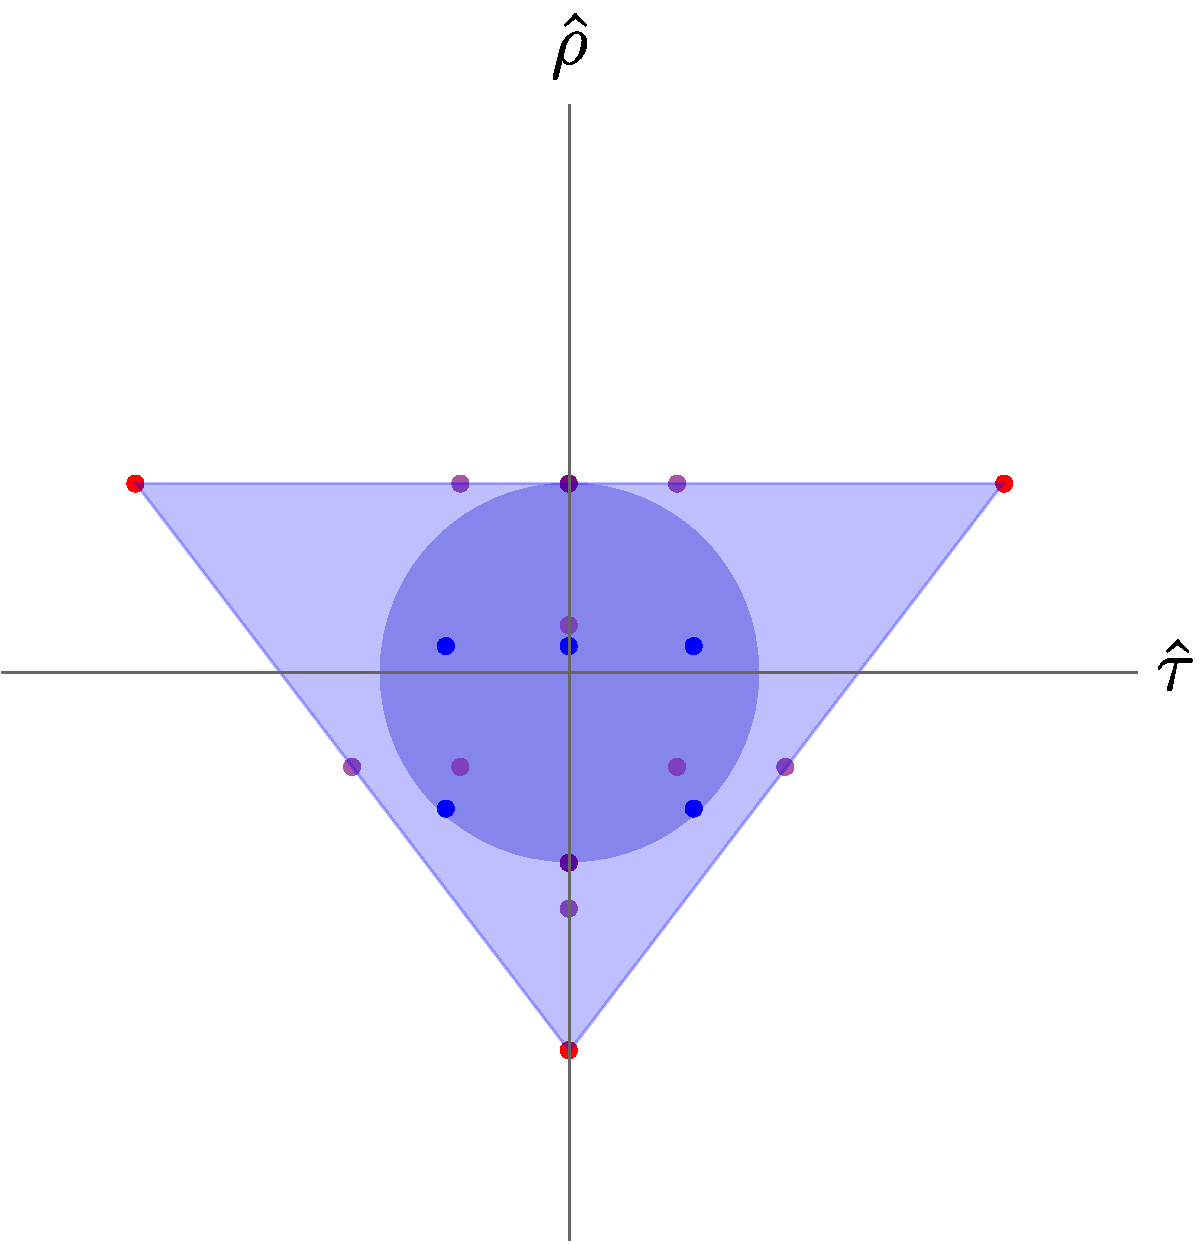
\includegraphics[width=0.45\textwidth]{CH-T3-projected.pdf}}\label{sfig:2dslice}
    \quad
	\subfigure[Toy model]{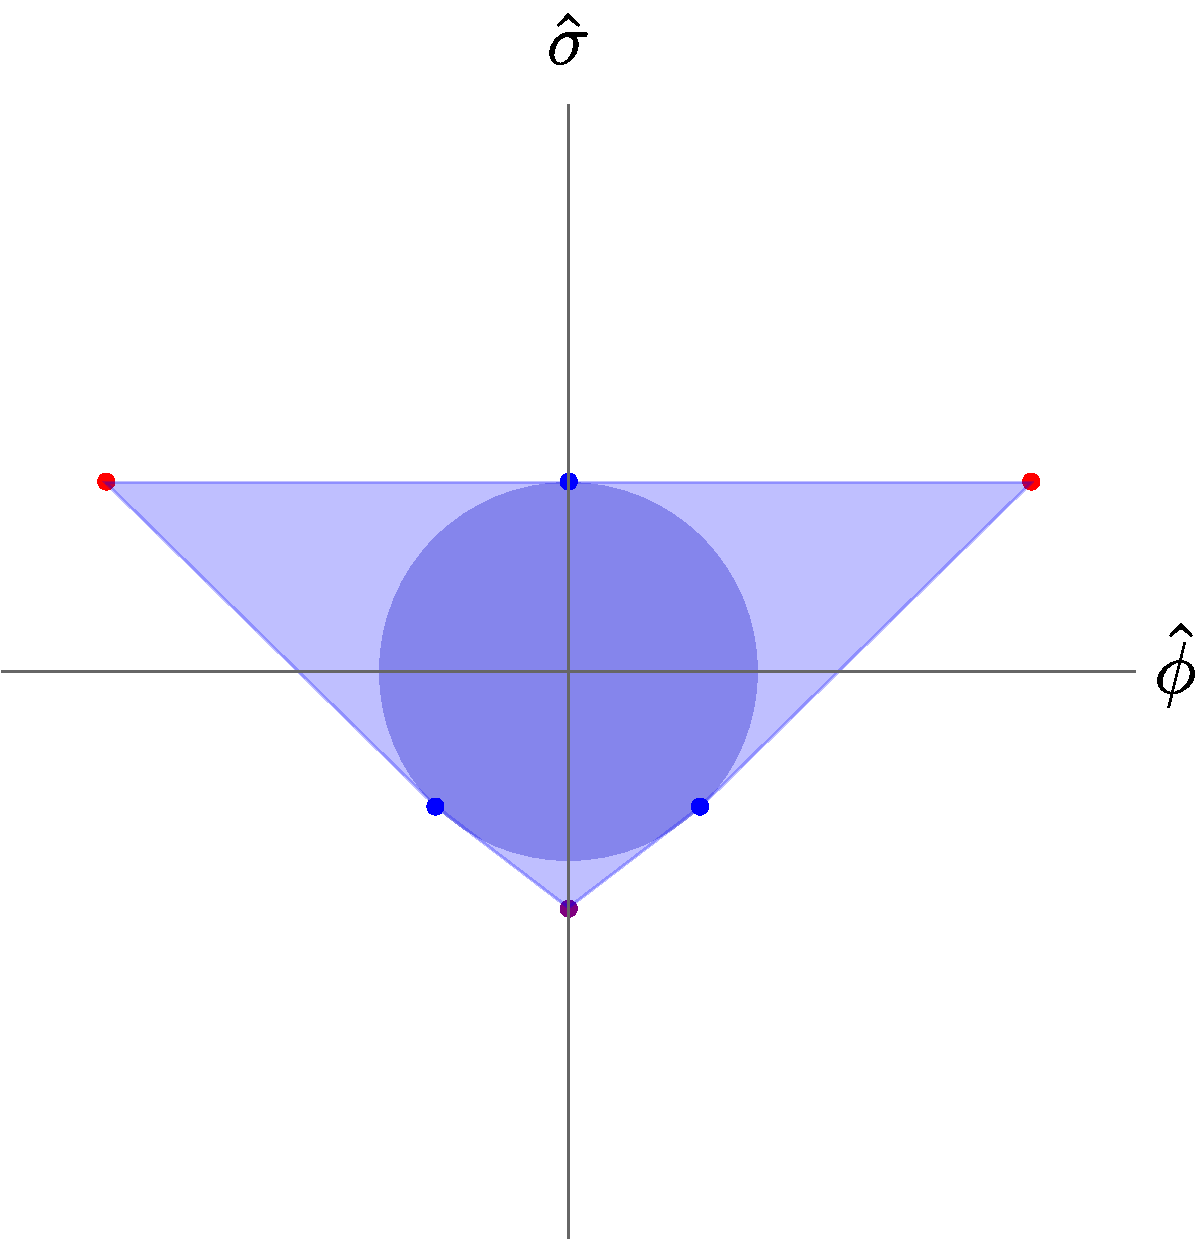
\includegraphics[width=0.45\textwidth]{CH-5.pdf}}\label{sfig:toymodel8d}
	\caption{\small \textbf{(a)} Two-dimensional projection of the convex hull for the species scale in M-theory on $\mathbf{T}^3$ along the plane perpendicular to $\hat T = \partial_{\hat{U}}$. \textbf{(b)} Convex hull diagram for the 9d $\to$ 8d compactification of the toy model discussed in Section \ref{ss:compactificationstring}.}
	\label{fig:ch-comparison-toymodel}	
\end{center}
\end{figure}
%%%%%%%%%%%%

\subsection{M-theory on $\mathbf{T}^k$}
\label{ss:MthyTk}

In this subsection we extend the results from the previous examples in nine and eight dimensions to M-theory compactifications on $\mathbf{T}^k$, for $k>3$. This will provide strong evidence in favour of the bound \eqref{eq:lowerboundspecies2} as well as the idea that there seems to exist a minimum rate at which the species scale can fall-off at infinity.

Our argument proceeds inductively, relying heavily both on U-duality (c.f. Section \ref{s:dualities}) and the uniqueness of the supergravity theory for $d<9$ spacetime dimensions. Crucially, U-duality forces all particle states comprising infinite towers with $p=1$ to arrange themselves into a \emph{single} irreducible representation of the symmetry group (see Table \ref{tab:irreps} below).\footnote{This is actually not true in 9d, where the KK-like towers form a $\mathbf{2} \oplus \mathbf{1}$ representation of the $\mathsf{SL(2, \mathbb{Z})}$ duality group. The reason for this hinges on the fact that there are two different limiting theories in ten dimensions with 32 supercharges one can arrive at from 9d, depending on their chirality\cite{Hull:1994ys}.} Such orbit includes both perturbative (i.e. KK, winding modes, etc.) and non-perturbative states (wrapped $p$-branes, KK-monopoles, etc.), as seen from the original duality frame. For instance, consider M-theory compactified on $\mathbf{T}^4$ down to 7d. The U-duality group is identified with $\mathsf{SL(5, \mathbb{Z})}$ in this case, and the particle multiplet transforms as the $\mathbf{10}$ of $\mathsf{SL(5, \mathbb{Z})}$. These states may be understood microscopically as four Kaluza-Klein towers associated to the compact directions, as well as six additional infinite sets of wrapped M2-particles.

Hence, we start with a couple of insights provided by the examples analyzed in Sections \ref{ss:MthyT2SSDC} and \ref{ss:MthyT3SSDC}. There we saw that the states with $p=1$ saturate the lower bound \eqref{eq:lowerboundspecies2}, and they appear precisely at the facets of the corresponding convex hull polytope. Furthermore, as already noticed, these facets turn out to be nothing but the convex hull of the theory in one dimension higher. Intuitively, this is easy to understand, since upon dimensionally reducing the supergravity theory, all $\mathcal{Z}$-vectors give rise to analogous ones combined with the KK tower associated to the extra circle. The latter generate the same polytope already existing in the higher-dimensional theory, which is moreover orthogonal to the species vector associated to decompactifying the new compact dimension, $\vec{\mathcal{Z}}_{\text{KK}}$ (see Section \ref{ss:field-theory} for details). Finally, the general analysis of Section \ref{s:consistencydimreduc} showed that if the theory we start with satisfies the CHC then, upon $\mathbf{S}^1$--\,compactification, we end up with a set of species vectors which still verify \eqref{eq:lowerboundspecies2} along all intermediate asymptotic directions.

With this we are now ready to argue that the condition \eqref{eq:lowerboundspecies2} is indeed satisfied in $d$-dimensional maximal supergravity for $d\geq4$. We work by induction, such that we first assume the bound to hold for M-theory compactified on $\mathbf{T}^k$, with species vectors denoted by $\{\vec{\mathcal{Z}}_{\text{t}}\}$. In a next step, we dimensionally reduce the theory on a circle, leading to M-theory on $\mathbf{T}^k \times \mathbf{S}^1 \cong \mathbf{T}^{k+1}$.\footnote{We freeze the axions to zero v.e.v., since as we learned from the previous examples they play no role whatsoever in our analysis (see Section \ref{ss:MthyT2SSDC}).} Based on the general considerations from the previous paragraph we conclude that the (sub-)polytope spanned by the set of vectors $\lbrace \vec{\mathcal{Z}}_{\text{KK}}, \vec{\mathcal{Z}}_{\text{KK-t},\, p+1}\rbrace$ satisfies the CHC, saturating the bound precisely along the direction determined by $\vec{\mathcal{Z}}_{\text{KK}}$ (c.f. equation \eqref{vectors}). However, from U-duality we know that this is already enough to ensure that the CHC holds in every asymptotic direction, since upon acting with the discrete remnant of the symmetry group, one can completely reconstruct the rest of the diagram. The latter presents as many identical facets as the dimension of the representation into which the $p=1$ towers fit into, which follows from the uniqueness of the supergravity action, at least for $d<9$. Therefore, by noticing that the condition \eqref{eq:lowerboundspecies2} was already shown to be satisfied in M-theory compactified on $\mathbf{T}^k$ for $k=1,2,3$, we thus conclude that the same remains true for maximal supergravity in lower dimensions as well.

\section{Summary}\label{s:summarybounds}

Let us summarize the main findings extracted from this chapter. First of all, we were able to determine a lower bound for the exponential decay rate $\lambda_{\rm sp}$ (c.f. eqs. \eqref{eq:defspeciesvectors}-\eqref{eq:decayratespecies} for a precise definition) of the quantum gravity cut-off close to infinite distance boundaries in field space, which only depends on the spacetime dimension of our theory. This translates into having a minimum rate at which the species scale can fall off with respect to the Planck mass at infinity, thereby forcing the exponential behaviour predicted by the Distance Conjecture \cite{Ooguri:2006in} when combined with other bounds proposed in the literature \cite{vandeHeisteeg:2023ubh, Calderon-Infante:2023ler}. Moreover, we were able to formulate this constraint in a manifestly reparametrization invariant way, namely in terms of a convex hull condition.

On the other hand, several interesting properties associated to the bound \eqref{eq:lowerboundspecies} were uncovered. In fact, we argued that the precise lowest possible value $ \frac{1}{\sqrt{(d-1)(d-2)}}$ is selected both empirically and by consistency with dimensional reduction, since it is the only one whose saturation is \emph{exactly} preserved by the compactification process. However, as typically happens with Swampland criteria, field-theoretic considerations do not suffice in general to ensure that the bound is satisfied for any possible infinite distance limit. This typically requires from the inclusion of additional extended objects in the theory, such as strings or higher-dimensional $p$-branes, as we readily confirmed with the examples discussed in Section \ref{s:examplesbound}.

In addition, we provided strong evidence for the constraint \eqref{eq:lowerboundspecies} via explicit verification in toroidal compactifications of M-theory, leading to maximal supergravity constructions in $d \geq 4$. This allowed us to extract further general lessons that we believe go beyond this highly-constrained systems. In particular, we observed that the convex hull diagrams were fully generated by string or Kaluza-Klein towers corresponding to full decompactification (i.e. back to 11d M-theory). This seems to capture the idea that, at the end of the day, we always expect the species scale to encode either the ten-dimensional string scale or the eleven-dimensional Planck mass. On the contrary, the species vectors signalling decompactification of just one extra dimension --- which therefore saturate the bound \eqref{eq:lowerboundspecies} --- were seen to lie always at the point closest to the origin within the different facets comprising the convex polytope. 

During the course of this investigation, we realized that the convex hulls associated to each of the examples analyzed so far exhibited rich geometric and symmetry casuistics, which are related to the duality properties of the theory. Furthermore, upon comparison with the convex hull determined by the tower scales, i.e. the $\zeta$-vectors (see discussion around eq. \eqref{eq:chargetomass} for details), we uncovered a non-trivial relation between the two. Indeed, the role of saturating/protecting towers for the corresponding lower bounds in the asymptotic exponential decay rates seemed to be exchanged. This hinges on some interesting mathematical duality relating both convex hull diagrams that will be further explored in the upcoming chapter.

